\documentclass[11pt,a4paper]{article}
\usepackage[utf8]{inputenc}
\usepackage[spanish]{babel}
\usepackage{geometry}
\geometry{margin=1in}
\usepackage{booktabs}
\usepackage{longtable}
\usepackage{graphicx}
\usepackage{float}
\usepackage{hyperref}
\usepackage{amsmath}
\usepackage{amssymb}
\usepackage{array}

\title{Reporte y Resumen Analítico de Artículos Científicos}
\date{\today}

\begin{document}

\maketitle
\tableofcontents
\newpage

\newpage
% --- Inicio del documento: A\_Novel\_Hilbert\_Antenna\_Enhanced\_With\_Metamaterials\_for\_Partial\_Discharge\_Detection.pdf ---
\section{A Novel Hilbert Antenna Enhanced With Metamaterials for Partial Discharge Detection}

\subsection*{Contexto y objetivo}
La detección de descargas parciales (PD, por sus siglas en inglés) es crucial para el mantenimiento y la seguridad de los equipos de alta tensión. Las antenas de ultra alta frecuencia (UHF) convencionales utilizadas para este fin adolecen de limitaciones significativas, como un tamaño físico excesivo y un ancho de banda estrecho. El presente estudio aborda estas limitaciones proponiendo un diseño novedoso de antena que busca expandir el ancho de banda sin aumentar las dimensiones físicas de la misma.

El objetivo principal de esta investigación es desarrollar una antena compacta con un ancho de banda amplio para la detección de PD en la banda UHF. Para lograrlo, se emplean dos estrategias:
\begin{enumerate}
    \item Integrar una curva fractal de Hilbert modificada en un diseño de antena espiral para ampliar el ancho de banda.
    \item Introducir una estructura de metamaterial simétrica de doble anillo abierto para mejorar aún más el rendimiento de la antena, incluyendo su ganancia, ancho de banda de detección y direccionalidad.
\end{enumerate}
La investigación busca validar el rendimiento de la antena propuesta tanto mediante simulaciones como experimentalmente.

\subsection*{Metodología o desarrollo}
El desarrollo de esta investigación se llevó a cabo en varias etapas, combinando el diseño de antenas fractales con metamateriales y su validación experimental.

\begin{enumerate}
    \item \textbf{Diseño de la antena espiral de Hilbert:}
    La antena espiral de Hilbert se diseñó integrando una curva fractal de Hilbert, conocida por sus propiedades de auto-similitud y llenado de espacio, en una disposición espiral rectangular. Esta integración permite excitar múltiples modos resonantes, ampliando el ancho de banda sin aumentar el tamaño físico.
    \begin{figure}[htpb]
    \centering
    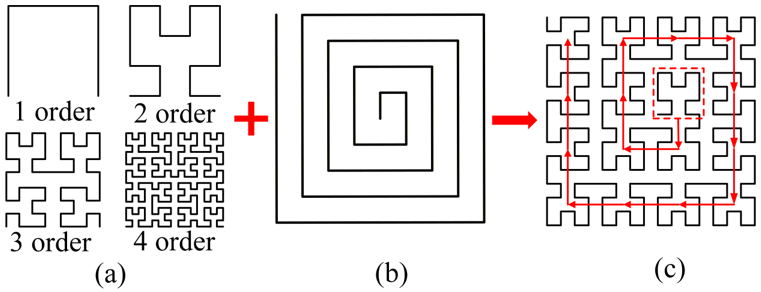
\includegraphics[width=0.8\textwidth]{images/80454576009ef7b4a427014bb7b6ca8c_p2_i1.png}
    \caption{Ideas de diseño para estructuras de antena espiral de Hilbert. (a) Curva de Hilbert. (b) Curva espiral rectangular. (c) Curva espiral de Hilbert.}
    \end{figure}
    Se realizó un estudio comparativo entre una antena espiral rectangular de 8 vueltas y una antena espiral de Hilbert de 2\textsuperscript{o} orden y 8 vueltas, ambas sobre un sustrato dieléctrico FR4 de 100 \texttimes\ 100 \texttimes\ 1.6 mm. Los resultados (ilustrados en \textbf{Figure 3}) mostraron que la antena espiral de Hilbert duplicaba el ancho de banda operativo (21.8\% vs. 9\%) para un VSWR $<$ 2.
    \begin{figure}[htpb]
    \centering
    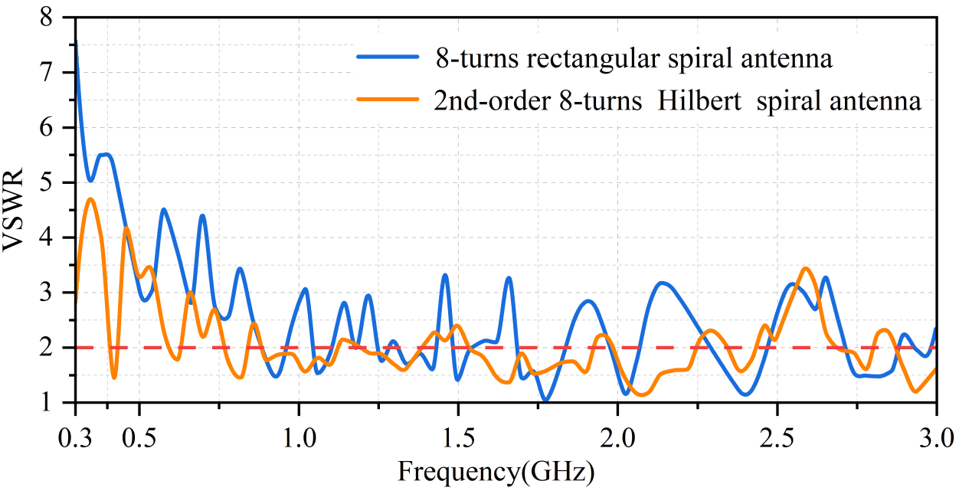
\includegraphics[width=0.8\textwidth]{images/80454576009ef7b4a427014bb7b6ca8c_p2_i2.png}
    \caption{Curvas de VSWR de la antena espiral de Hilbert de 2\textsuperscript{o} orden y ocho vueltas y la antena espiral rectangular de ocho vueltas.}
    \end{figure}
    A través de un análisis paramétrico de diferentes órdenes fractales y números de vueltas (detallado en \textbf{Table I} del documento original), se seleccionó la antena espiral de Hilbert de 2\textsuperscript{o} orden y cuatro vueltas como el diseño final, que ofrecía un ancho de banda operacional del 56.7\% en la banda UHF.

    \item \textbf{Diseño de la unidad de metamaterial:}
    Para mejorar el ancho de banda del 56.7\% de la antena espiral de Hilbert, se introdujo una estructura de metamaterial (MM) consistente en una unidad simétrica de doble anillo abierto con un diseño espiral continuamente curvado. Este diseño se basa en la teoría de resonancia LC (\textbf{ecuación 1} del documento), optimizando la inductancia y capacitancia equivalentes para reducir la frecuencia resonante fundamental sin aumentar el tamaño.
    \begin{figure}[htpb]
    \centering
    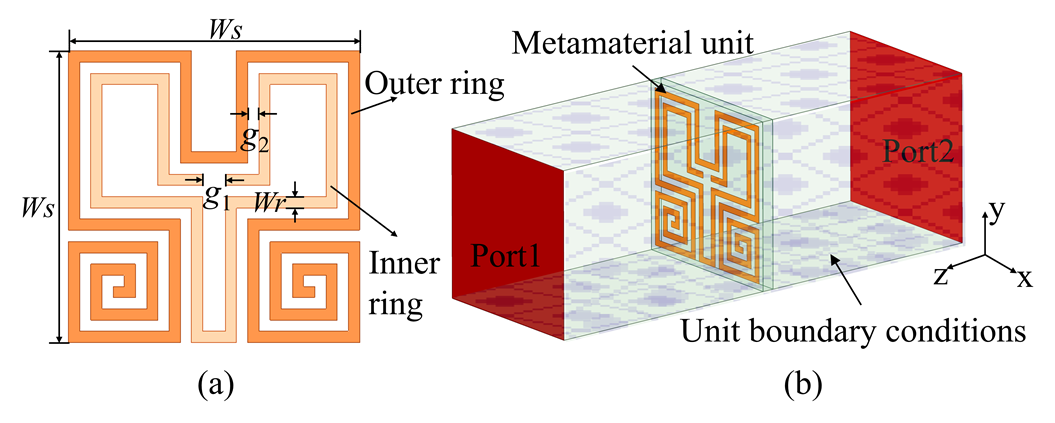
\includegraphics[width=0.8\textwidth]{images/80454576009ef7b4a427014bb7b6ca8c_p3_i1.png}
    \caption{(a) Estructura de la unidad de metamaterial y (b) esquema de simulación del puerto Floquet.}
    \end{figure}
    Las simulaciones electromagnéticas de onda completa se realizaron utilizando CST Studio Suite, aplicando el método de puerto Floquet. Se llevó a cabo una optimización paramétrica variando el ancho de línea (\textit{wr}), el ancho de la brecha interna (\textit{g1}) y el ancho de la brecha entre anillos (\textit{g2}) para analizar su influencia en la curva S21 (como se muestra en \textbf{Figure 5} del documento original, partes (a), (b) y (c)).
    \begin{figure}[htpb]
    \centering
    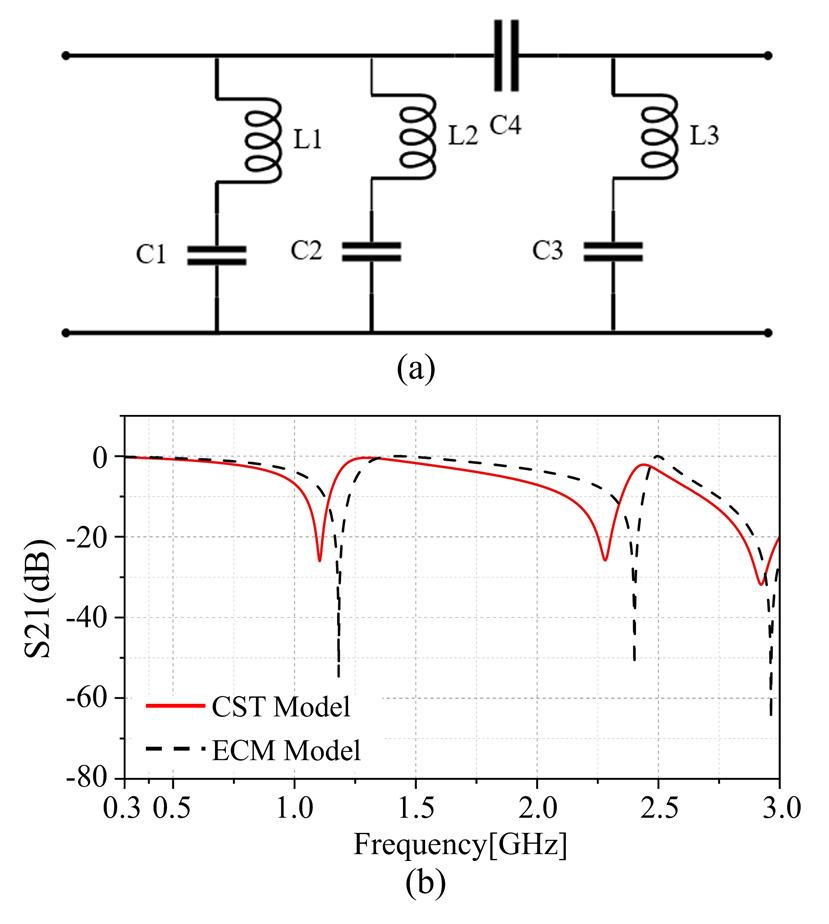
\includegraphics[width=0.8\textwidth]{images/80454576009ef7b4a427014bb7b6ca8c_p4_i1.png}
    \caption{Curva S21 obtenida al cambiar $w_r$.}
    \end{figure}
    \begin{figure}[htpb]
    \centering
    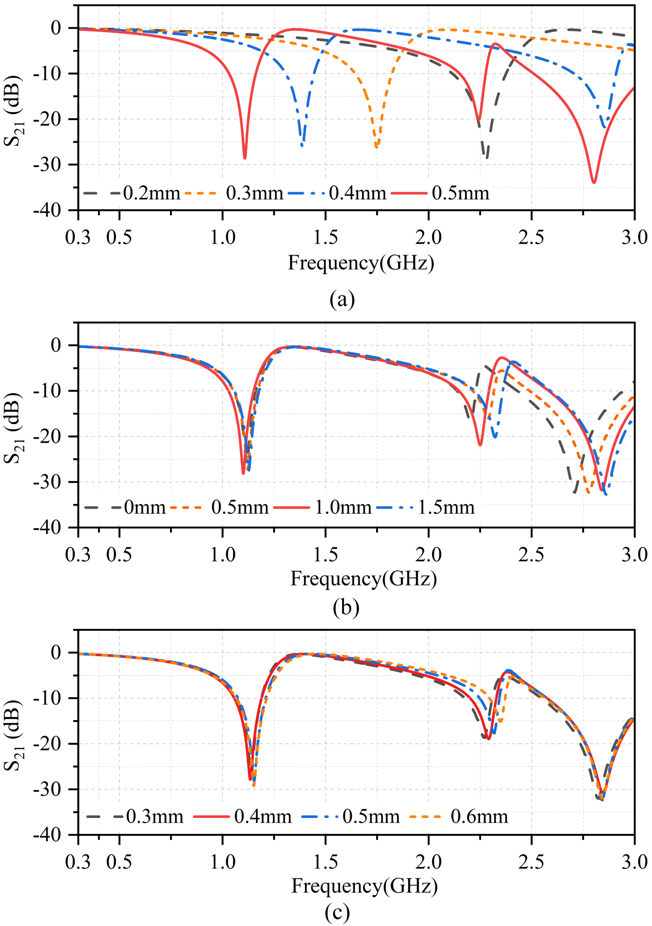
\includegraphics[width=0.8\textwidth]{images/80454576009ef7b4a427014bb7b6ca8c_p4_i2.png}
    \caption{Curva S21 obtenida al cambiar $g_1$.}
    \end{figure}
    \begin{figure}[htpb]
    \centering
    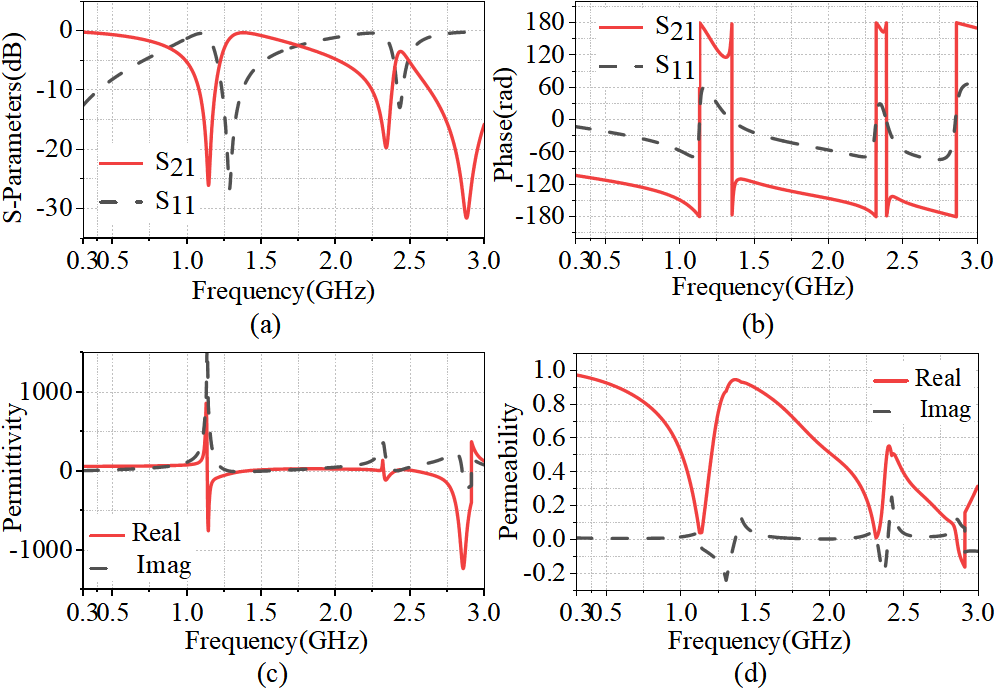
\includegraphics[width=0.8\textwidth]{images/80454576009ef7b4a427014bb7b6ca8c_p4_i3.png}
    \caption{Curva S21 obtenida al cambiar $g_2$.}
    \end{figure}
    Los parámetros finales optimizados fueron: $ws = 13$ mm, $wr = 0.5$ mm, $g1 = 1$ mm y $g2 = 0.4$ mm. Se desarrolló un modelo de circuito equivalente para caracterizar el mecanismo de transmisión de ondas electromagnéticas, validado por simulaciones de onda completa (detallado en \textbf{Figure 7} del documento original, que no se incluye en esta respuesta).

    \item \textbf{Integración de metamateriales en la antena:}
    El metamaterial se dispuso en un arreglo de 8 \texttimes\ 8 unidades a una altura $d_1$ por encima de la antena espiral de Hilbert, fabricado sobre un sustrato FR4. El principio es modificar la trayectoria de propagación de las ondas electromagnéticas, permitiendo que la antena capture más señales entrantes y mejore su sensibilidad (\textbf{Figure 8}).
    \begin{figure}[htpb]
    \centering
    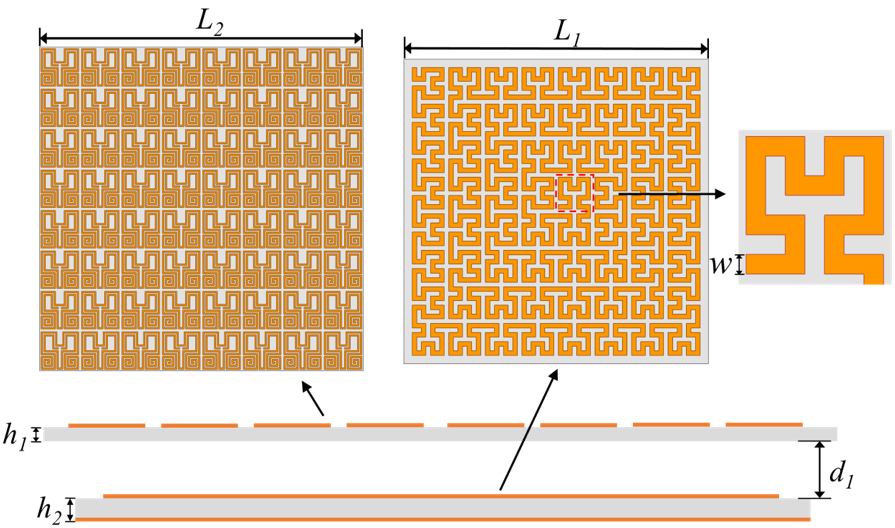
\includegraphics[width=0.8\textwidth]{images/80454576009ef7b4a427014bb7b6ca8c_p5_i1.png}
    \caption{Trayectoria de propagación de ondas electromagnéticas a través de la placa de metamaterial.}
    \end{figure}
    Se realizó una optimización de la distancia $d_1$ entre el arreglo de metamaterial y la antena, con simulaciones para $d_1$ = 10, 20, 30 y 40 mm (\textbf{Figure 10}). El valor óptimo de $d_1$ se determinó en 10 mm.
    \begin{figure}[htpb]
    \centering
    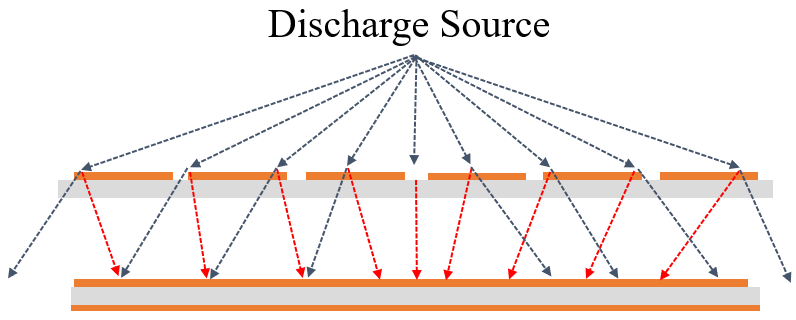
\includegraphics[width=0.8\textwidth]{images/80454576009ef7b4a427014bb7b6ca8c_p5_i2.png}
    \caption{Estructura general de la antena espiral de Hilbert con metamateriales.}
    \end{figure}
    \begin{figure}[htpb]
    \centering
    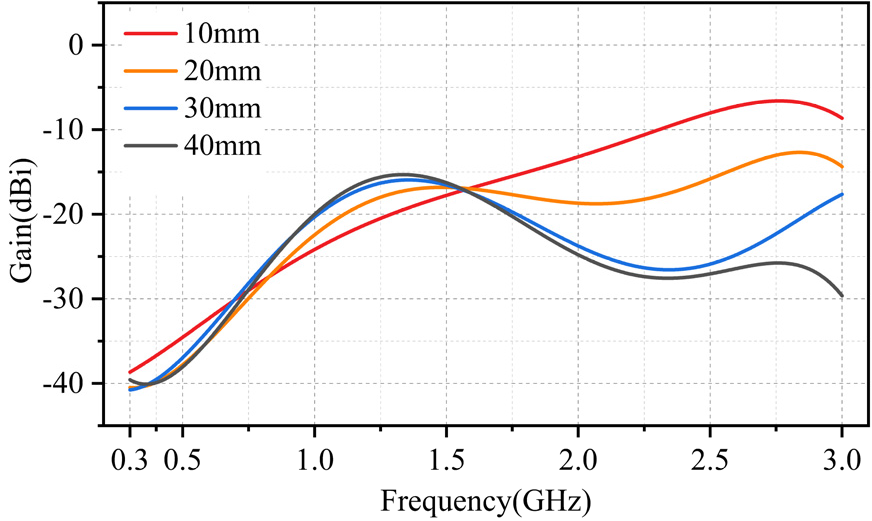
\includegraphics[width=0.8\textwidth]{images/80454576009ef7b4a427014bb7b6ca8c_p5_i3.png}
    \caption{Ganancia a diferentes distancias entre el arreglo de metamaterial y la antena.}
    \end{figure}

    \item \textbf{Pruebas de antenas y metamateriales:}
    Tras las simulaciones, la antena diseñada y el arreglo de metamaterial se fabricaron en una placa de circuito impreso (PCB). Se validó experimentalmente su rendimiento utilizando el método de medición en espacio libre para los parámetros S, VSWR y ganancia. El sistema experimental (\textbf{Figure 14}) utiliza una antena transmisora, la placa de metamaterial, la antena receptora y un analizador vectorial de redes (VNA).
    \begin{figure}[htpb]
    \centering
    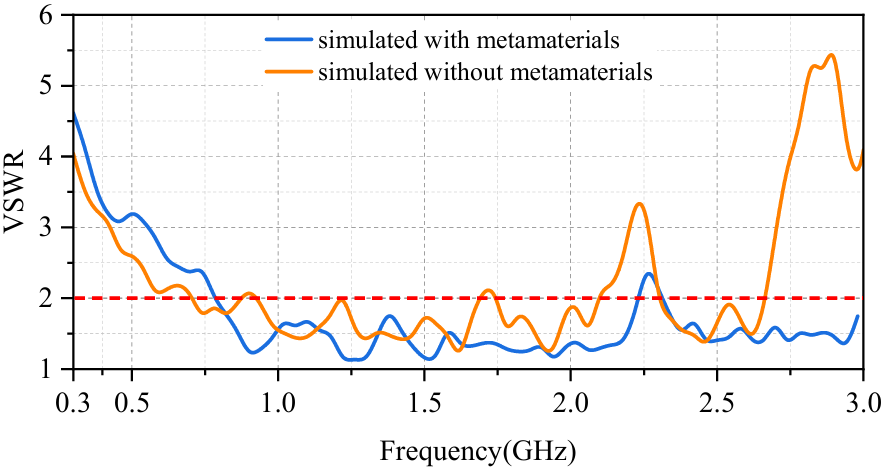
\includegraphics[width=0.8\textwidth]{images/80454576009ef7b4a427014bb7b6ca8c_p6_i4.png}
    \caption{(a) Medición de parámetros S de metamateriales por el método de espacio libre. (b) Diagrama de medición in situ por el método de espacio libre.}
    \end{figure}
    Finalmente, se construyó un sistema de detección de PD en laboratorio para evaluar la capacidad de la antena de detectar señales de PD. Este sistema (\textbf{Figure 18}) incluía un transformador, un resistor limitador, un aislante compuesto (contaminado artificialmente), un osciloscopio y dos antenas (con y sin metamateriales), junto con amplificadores de bajo ruido.
    \begin{figure}[htpb]
    \centering
    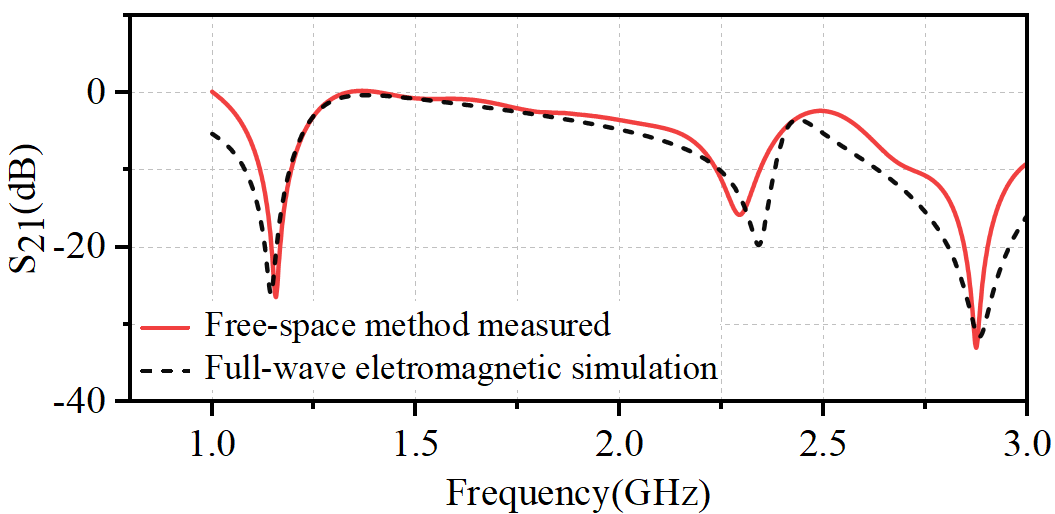
\includegraphics[width=0.8\textwidth]{images/80454576009ef7b4a427014bb7b6ca8c_p7_i8.png}
    \caption{(a) Diagrama del sistema de detección de PD.}
    \end{figure}
    \begin{figure}[htpb]
    \centering
    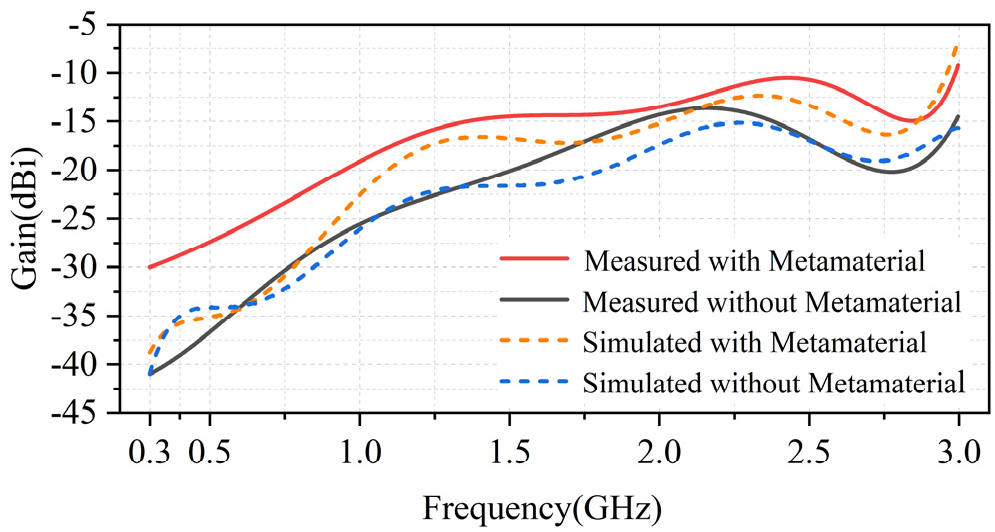
\includegraphics[width=0.8\textwidth]{images/80454576009ef7b4a427014bb7b6ca8c_p7_i9.png}
    \caption{(b) Disposición del sitio experimental.}
    \end{figure}
    \begin{figure}[htpb]
    \centering
    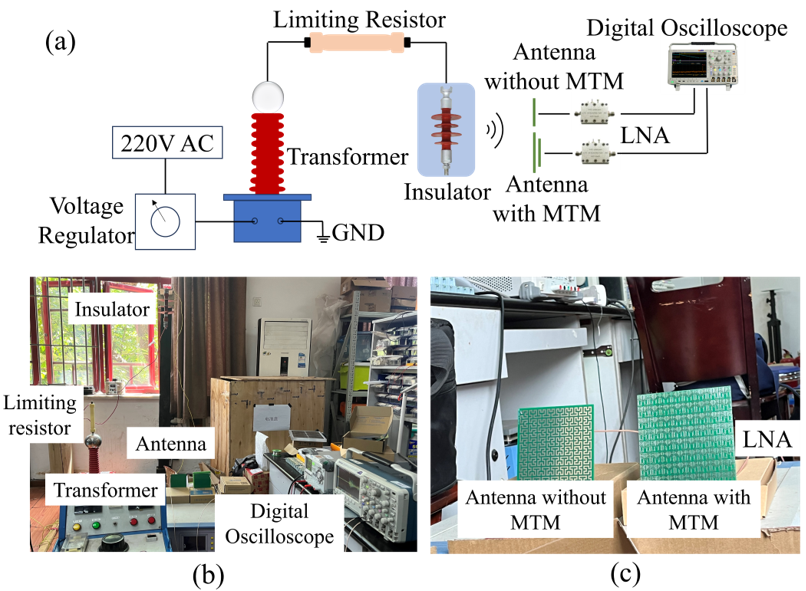
\includegraphics[width=0.8\textwidth]{images/80454576009ef7b4a427014bb7b6ca8c_p7_i10.png}
    \caption{(c) Disposición de la antena en el experimento de campo.}
    \end{figure}
    Se midieron las señales de PD a diferentes distancias (2-10 m) para ambas configuraciones de antena (con y sin metamateriales), y se calcularon las amplitudes de pulso promedio (APA) para cuantificar la sensibilidad de detección (según la \textbf{ecuación 8} del documento).
\end{enumerate}

\subsection*{Resultados o hallazgos}
Los resultados de este estudio demuestran mejoras significativas en el rendimiento de la antena:
\begin{enumerate}
    \item \textbf{Antena espiral de Hilbert (diseño base):} El diseño de 2\textsuperscript{o} orden y 4 vueltas de la antena espiral de Hilbert logró un ancho de banda operativo del 56.7\% en la banda UHF para un VSWR $<$ 2.

    \item \textbf{Rendimiento de la unidad de metamaterial:} La unidad de metamaterial exhibió tres ceros de transmisión a 1.1, 2.25 y 2.9 GHz. Mostró permisividad negativa en rangos de frecuencia de 1.13-1.35 GHz, 2.32-2.39 GHz y 2.56-2.91 GHz, y simultáneamente permisividad y permeabilidad negativas en el rango de 2.86-2.91 GHz. El modelo de circuito equivalente desarrollado se validó con éxito mediante simulaciones de onda completa (resultados de la \textbf{Figure 6} y \textbf{Figure 7} del documento original, no incluidas en esta respuesta).

    \item \textbf{Antena con metamateriales (simulación):}
    % [Imagen omitida porque no se encontró el archivo: 80454576009ef7b4a427014bb7b6ca8c_p11_i1.png]
    Comparando la antena sin y con metamateriales, la configuración integrada logró un VSWR $<$ 2 en dos bandas de frecuencia amplias: 0.78-2.02 GHz y 2.22-3 GHz. Esto representa un aumento del 24.4\% en el ancho de banda operacional. Se observó una mejora promedio de la ganancia de 4.61 dBi (\textbf{Figure 10}). La directividad y el rendimiento de radiación se vieron significativamente mejorados, con una concentración de la energía radiada (\textbf{Figure 12}).
    \begin{figure}[htpb]
    \centering
    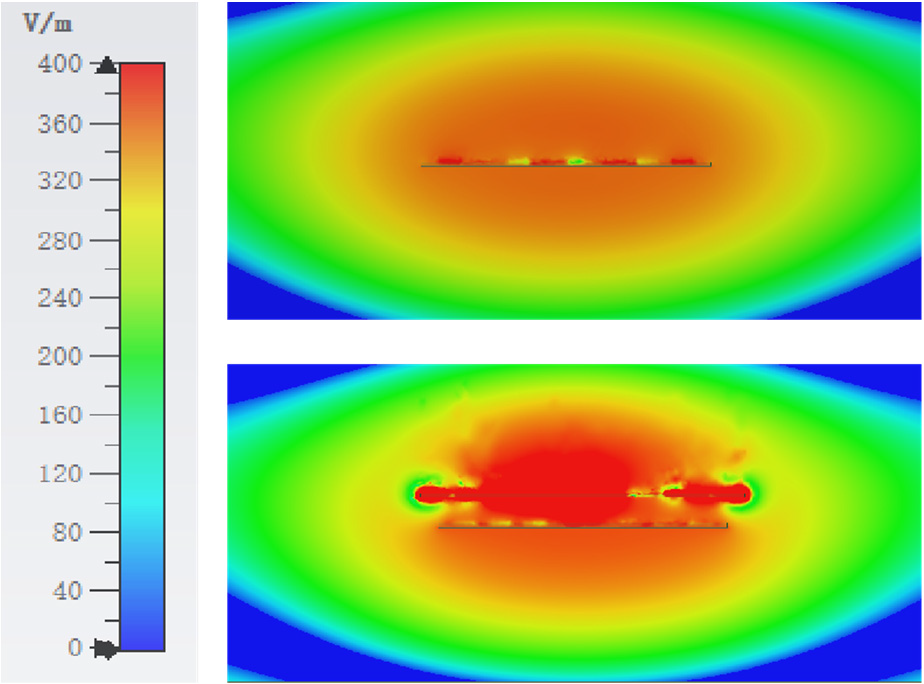
\includegraphics[width=0.8\textwidth]{images/80454576009ef7b4a427014bb7b6ca8c_p6_i2.png}
    \caption{Dirección de radiación con y sin metamateriales de mejora a 1.1, 2.25 y 2.9 GHz.}
    \end{figure}
    La distribución del campo eléctrico (\textbf{Figure 13}) mostró que el metamaterial concentra y refuerza eficazmente el campo eléctrico, optimizando la trayectoria de propagación de ondas electromagnéticas y mejorando la eficiencia de radiación.
    \begin{figure}[htpb]
    \centering
    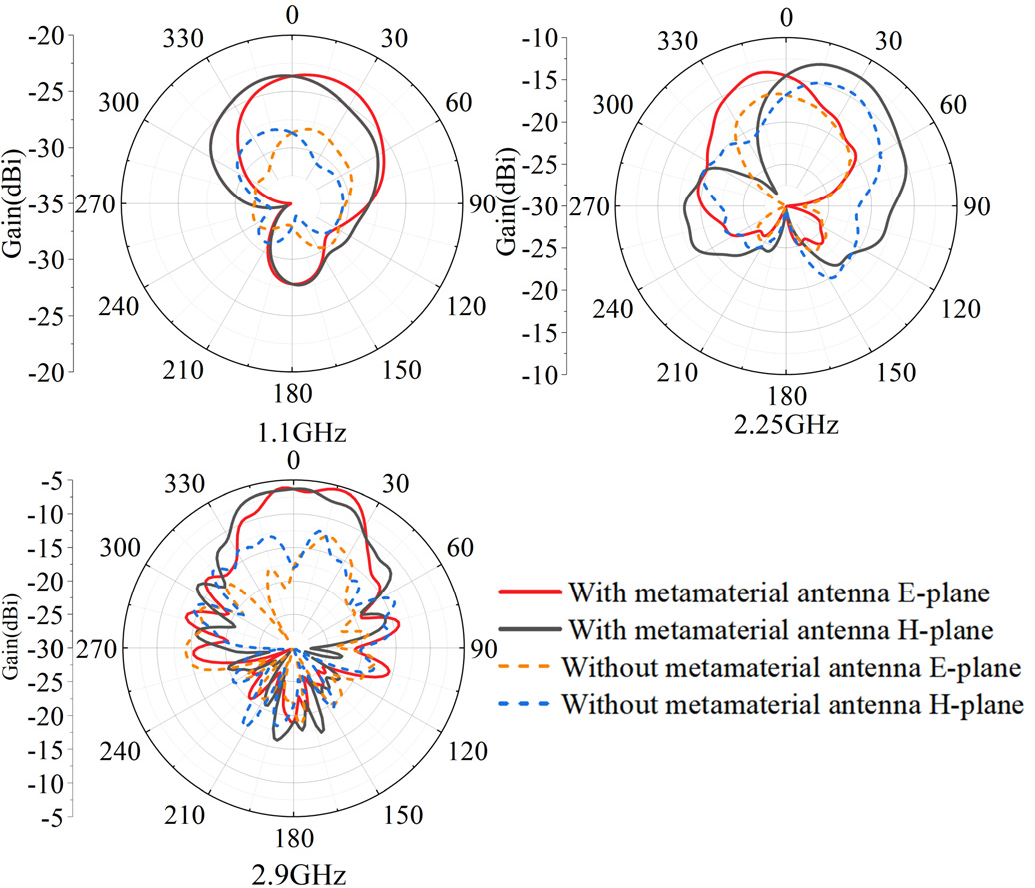
\includegraphics[width=0.8\textwidth]{images/80454576009ef7b4a427014bb7b6ca8c_p6_i3.png}
    \caption{Distribución del campo eléctrico con y sin metamaterial.}
    \end{figure}

    \item \textbf{Resultados de la validación experimental:}
    Las mediciones en espacio libre del parámetro S21 confirmaron la precisión de las simulaciones. Las curvas de VSWR y ganancia experimentales (mostradas en las \textbf{Figure 16} y \textbf{Figure 17} del documento original, no incluidas en esta respuesta) también se alinearon con los resultados simulados, validando el aumento del 24.4\% en el ancho de banda de detección y la mejora de la ganancia promedio de 4.61 dBi.
    En las pruebas de detección de PD (cuyas formas de onda y espectros de dominio temporal se presentan en las \textbf{Figure 19} y \textbf{Figure 20} del documento original, no incluidas aquí), la antena con metamateriales mostró una sensibilidad de detección 125\% mayor que la antena sin metamateriales a distancias de 2-8 m (según \textbf{Table III} del documento original). Además, el rango de detección de la antena con metamateriales se expandió hasta 10 m.
\end{enumerate}

\subsection*{Discusión o análisis crítico}
Este estudio aborda con éxito las limitaciones de tamaño y ancho de banda de las antenas UHF convencionales para la detección de PD. La integración de la curva fractal de Hilbert en el diseño espiral es una estrategia eficaz para lograr una mayor densidad de circuito y, por ende, un ancho de banda más amplio en un formato compacto. La naturaleza auto-similar y de llenado de espacio de los fractales de Hilbert permite resonancias multifrecuencia, lo que es esencial para cubrir el espectro amplio de las señales de PD.

La adición del metamaterial es la contribución clave para potenciar aún más el rendimiento de la antena. La estructura de doble anillo abierto con diseño espiral, operando bajo la teoría de resonancia LC, manipula eficazmente las ondas electromagnéticas. Al concentrar y reforzar el campo eléctrico, el metamaterial no solo amplía significativamente el ancho de banda y la ganancia, sino que también mejora la directividad de la antena. Esto se traduce en una mayor capacidad para capturar señales de PD, incluso débiles, y discernir su dirección.

La comparación con antenas reportadas en la literatura (\textbf{Table IV} del documento original) destaca que la antena propuesta es significativamente más compacta (100 \texttimes\ 100 \texttimes\ 1.6 mm) y logra un ancho de banda proporcional del 81.1\% en la banda UHF, superando la mayoría de los diseños existentes en términos de eficiencia de espacio y cobertura de frecuencia. Aunque la ganancia intrínseca de la antena es moderada debido a su tamaño compacto, la inclusión de amplificadores de bajo ruido en el sistema de detección compensa esta limitación, permitiendo un alcance de detección de 10 m.

Una limitación reconocida es que las pruebas experimentales se realizaron únicamente con aisladores. Sin embargo, el bajo coste de fabricación (sustrato FR4 y capa de microtira de cobre) y el diseño compacto la hacen atractiva para futuras aplicaciones de monitoreo en línea en equipos de alta tensión como GIS (sistemas de aislamiento de gas), transformadores y otros dispositivos complejos. La versatilidad de la matriz de metamateriales también sugiere su posible aplicación para mejorar otras antenas.

\subsection*{Conclusiones o implicaciones}
Este estudio presenta una solución innovadora y eficaz para la detección de descargas parciales (PD) en equipos de alta tensión. Se demuestra que la combinación de una antena espiral basada en la curva fractal de Hilbert y un arreglo de metamateriales es una estrategia robusta para superar las limitaciones de las antenas UHF convencionales.

El diseño de la antena espiral de Hilbert de 2\textsuperscript{o} orden y 4 vueltas es intrínsecamente compacto (100 \texttimes\ 100 \texttimes\ 1.6 mm) y proporciona un ancho de banda operativo del 56.7\%. La integración de un arreglo de metamateriales de doble anillo abierto y simétrico, colocado 10 mm por encima de la antena, amplía este ancho de banda en un 24.4\%, abarcando las bandas de 0.78-2.02 GHz y 2.22-3 GHz. Esta configuración también mejora la ganancia promedio en 4.61 dBi y aumenta la directividad, concentrando la energía del campo eléctrico y optimizando la trayectoria de propagación de las ondas.

Los resultados experimentales validan las simulaciones, mostrando una sensibilidad de detección 125\% mayor y un rango de detección extendido a 10 m para la antena con metamateriales, en comparación con el diseño sin metamateriales. Estas características la hacen altamente adecuada para el monitoreo en línea de PD, especialmente en espacios confinados como los encontrados en los GIS. La metodología y los hallazgos tienen implicaciones significativas para el desarrollo de futuras tecnologías de detección de PD más eficientes y compactas.

\subsection*{Síntesis final}
Este estudio presenta una antena espiral de Hilbert innovadora y compacta para la detección de descargas parciales (PD). La integración de un arreglo de metamateriales de doble anillo abierto mejora significativamente el ancho de banda en un 24.4\%, la ganancia promedio en 4.61 dBi y la directividad. Las simulaciones y experimentos confirman una sensibilidad de detección 125\% mayor y un alcance de 10 m, haciendo de esta antena una solución prometedora para el monitoreo en línea de equipos de alta tensión.

\newpage
% --- Inicio del documento: Miniaturized\_Broadband\_Antenna\_Loaded\_With\_Frequency\_Selective\_Surface\_for\_Corona\_Discharge\_Detection.pdf ---
\section{Miniaturized Broadband Antenna Loaded With Frequency Selective Surface for Corona Discharge Detection}

\subsection*{Contexto y objetivo}
La descarga de corona es un fenómeno común en líneas de transmisión de alto voltaje, que provoca daños en el aislamiento y pérdidas de energía. Los métodos de detección actuales, como las antenas, tienen una sensibilidad limitada que impide la identificación precisa de la ubicación de las descargas. Los diseños de antenas existentes son a menudo grandes (e.g., 2x4 m o 360 mm de diámetro) y solo pueden detectar la presencia o ausencia de corona, sin determinar la ubicación exacta, lo que limita su uso con vehículos aéreos no tripulados (UAV). Trabajos previos han demostrado que la superposición de una Superficie Selectiva en Frecuencia (FSS) en una antena puede mejorar su capacidad para capturar ondas electromagnéticas.

El objetivo principal de este estudio es diseñar una FSS miniaturizada de banda ancha que opere en el rango de frecuencia de descarga de corona (100–500 MHz) para mejorar la sensibilidad y la distancia de detección de las antenas, permitiendo una detección más precisa y segura de las descargas de corona, especialmente para aplicaciones con UAVs.

\subsection*{Metodología o desarrollo}
El estudio se dividió en varias fases: diseño de la FSS, simulación de la antena y experimentos de detección de descarga de corona.

\textbf{1. Diseño de la Superficie Selectiva en Frecuencia (FSS):}
\begin{itemize}
    \item \textbf{Requisitos de diseño:} La FSS fue diseñada para operar entre 100 y 500 MHz, donde la energía de la señal de descarga de corona es más pronunciada y el ruido es bajo. Se requirió un valor de S11 < -10 dB para absorber más del 90\% de la onda electromagnética incidente y un tamaño de celda pequeño para evitar lóbulos de rejilla.
    \item \textbf{Evolución de la celda FSS:} El diseño comenzó con una celda cruzada básica, la cual fue mejorada al doblar y extender los extremos de los cuatro brazos en ángulos de 90° para formar una estructura serpentina. Esta evolución gradual, como se muestra en la Figura \ref{fig:fss_evolution}, buscó reducir la frecuencia resonante.
    \begin{figure}[htpb]
    \centering
    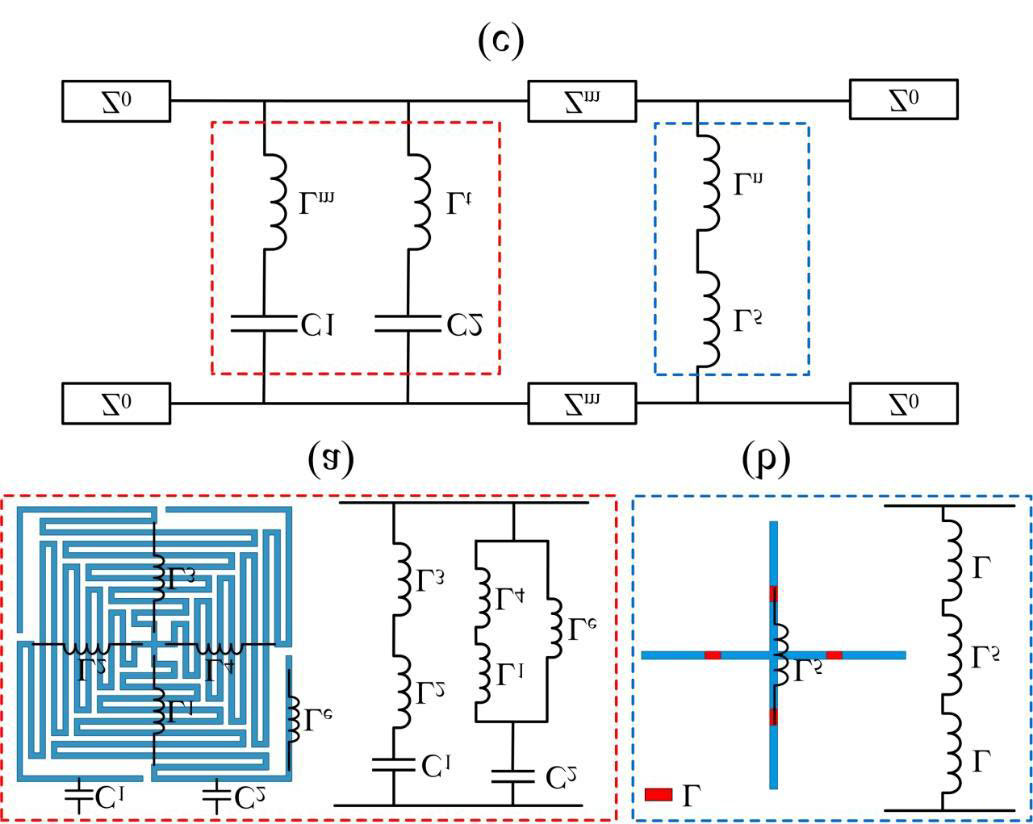
\includegraphics[width=0.8\textwidth]{images/564630268a062c85fb92b70f0c2f667c_p3_i1.jpeg}
    \caption{Proceso de conversión de la FSS de capa única de señal.}
    \end{figure}
    \item \textbf{Diseño de doble capa:} Se añadió un parche metálico en la parte posterior del sustrato dieléctrico para formar una FSS de doble capa, con la parte inferior con componentes inductivos para reducir aún más la frecuencia resonante. La celda FSS final (Figura \ref{fig:final_fss}) tiene dimensiones de 10 x 10 x 1.6 mm.
    \begin{figure}[htpb]
    \centering
    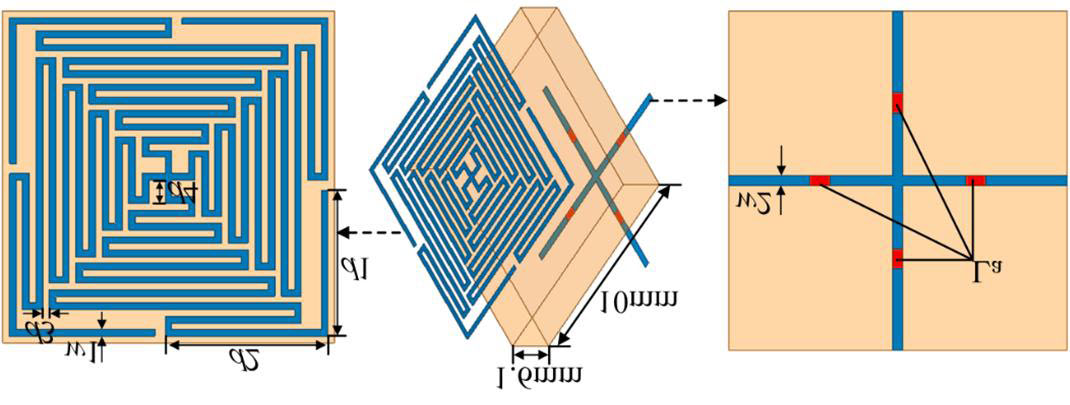
\includegraphics[width=0.8\textwidth]{images/564630268a062c85fb92b70f0c2f667c_p4_i5.jpeg}
    \caption{Estructura general de la FSS finalizada.}
    \end{figure}
    \item \textbf{Circuito equivalente:} Se construyó un circuito equivalente para analizar el comportamiento de la FSS (Figura \ref{fig:equivalent_circuit}), identificando capacitores (C1, C2) y bobinas (L1, L2, L3, L4, Lm, Ln, Ls) basadas en la distribución del campo eléctrico y la corriente superficial.
    \begin{figure}[htpb]
    \centering
    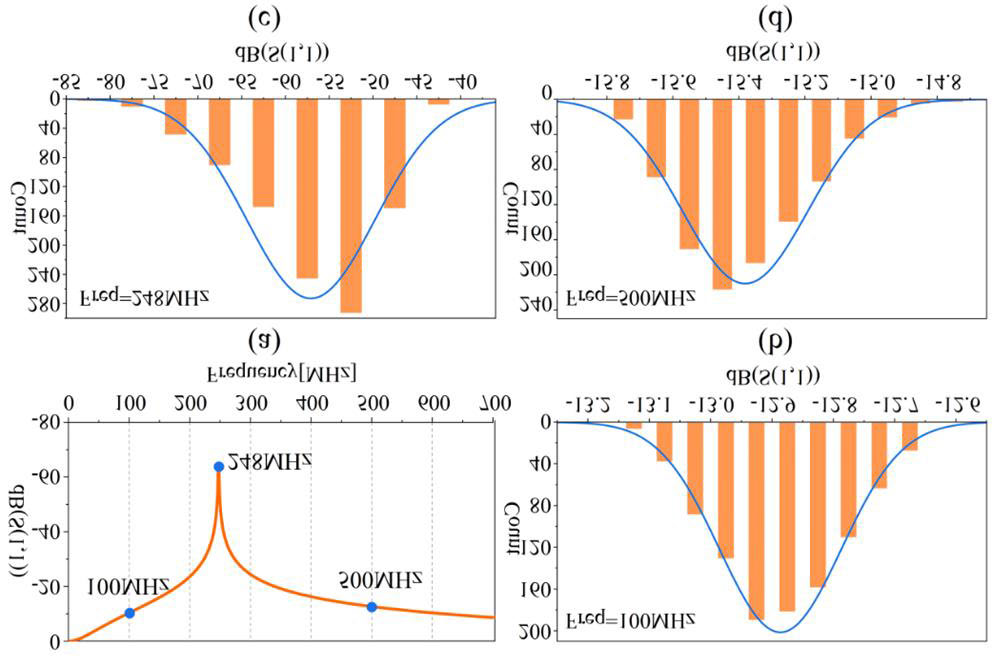
\includegraphics[width=0.8\textwidth]{images/564630268a062c85fb92b70f0c2f667c_p4_i1.jpeg}
    \caption{(a) Circuito equivalente del parche metálico superior. (b) Celda cruzada y circuito equivalente del inductor de chip cargado. (c) Circuito equivalente finalizado.}
    \end{figure}
    \item \textbf{Análisis de Monte Carlo:} Se realizó un análisis de Monte Carlo utilizando ANSYS para evaluar el impacto de las tolerancias de ±5\% en el valor de la inductancia del chip (390 nH nominal) en el rendimiento S11 de la FSS.
\end{itemize}

\textbf{2. Simulación y Análisis de Antenas:}
\begin{itemize}
    \item \textbf{Antena de detección:} Se utilizó una antena fractal de Hilbert serpentina (SHU) preexistente de 130 × 130 × 1.6 mm como antena de detección.
    \item \textbf{Superposición de FSS:} La FSS diseñada se colocó sobre la antena SHU (formando la antena FSHU), y se simuló la distancia óptima 'h' entre la FSS y la antena. Se probaron alturas de 10, 20, 30 y 40 mm. El principio de operación se muestra en la Figura \ref{fig:fss_principle}.
    \begin{figure}[htpb]
    \centering
    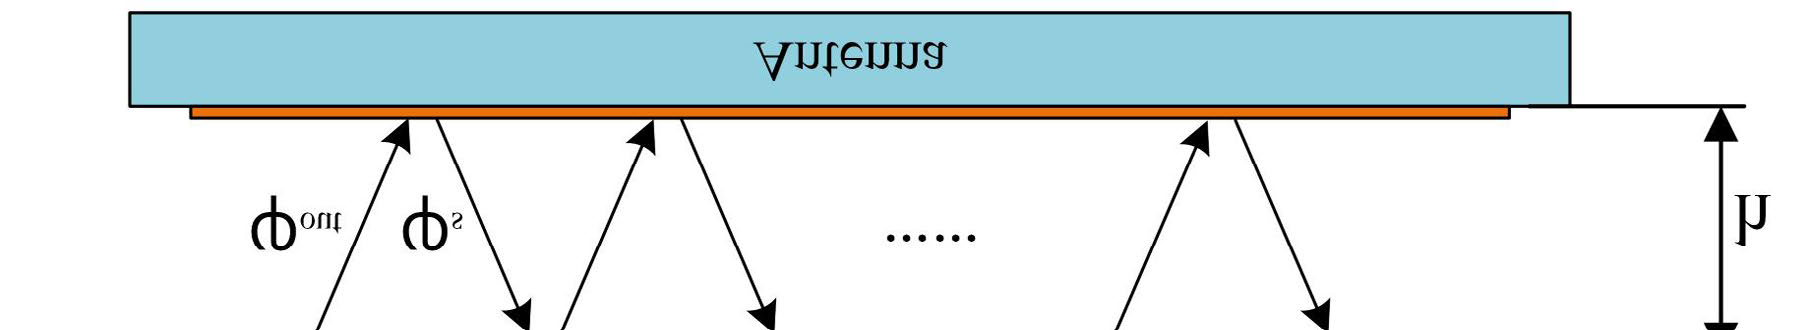
\includegraphics[width=0.8\textwidth]{images/564630268a062c85fb92b70f0c2f667c_p2_i3.jpeg}
    \caption{Principio de funcionamiento de la matriz FSS en antenas apiladas.}
    \end{figure}
    \item \textbf{Configuración de límites:} Se utilizaron configuraciones de límites específicas en las simulaciones (puertos floquet, límites maestro-esclavo) para la FSS y límites radiantes para la antena FSHU.
\end{itemize}

\textbf{3. Experimentos de Detección de Descarga de Corona:}
\begin{itemize}
    \item \textbf{Fabricación:} Se fabricaron prototipos de la antena SHU y la matriz FSS utilizando tecnología PCB estándar y técnicas de colocación de máquinas (Figura \ref{fig:fabricated_antennas}).
    \begin{figure}[htpb]
    \centering
    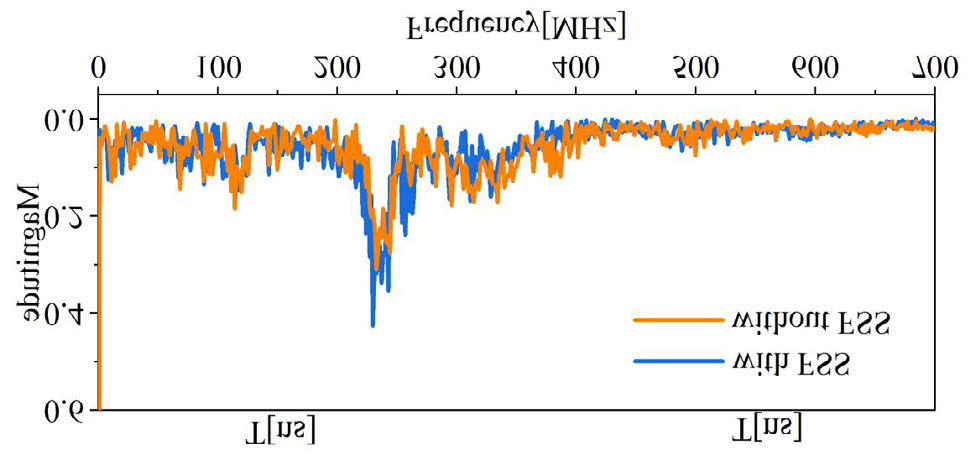
\includegraphics[width=0.8\textwidth]{images/564630268a062c85fb92b70f0c2f667c_p7_i2.jpeg}
    \caption{(c) Antena SHU física. (d) Comparación de la curva S11 medida con la simulación.}
    \end{figure}
    \item \textbf{Plataforma experimental:} Se montó una plataforma de prueba (Figura \ref{fig:experimental_platform}) que incluía un sistema transformador de 10 kA/50 kV, aisladores compuestos con contaminación artificial, las antenas SHU y FSHU, filtros de paso de banda (100-500 MHz), un amplificador de bajo ruido (LNA) y un osciloscopio multicanal (RIGOL MSO2202A).
    \begin{figure}[htpb]
    \centering
    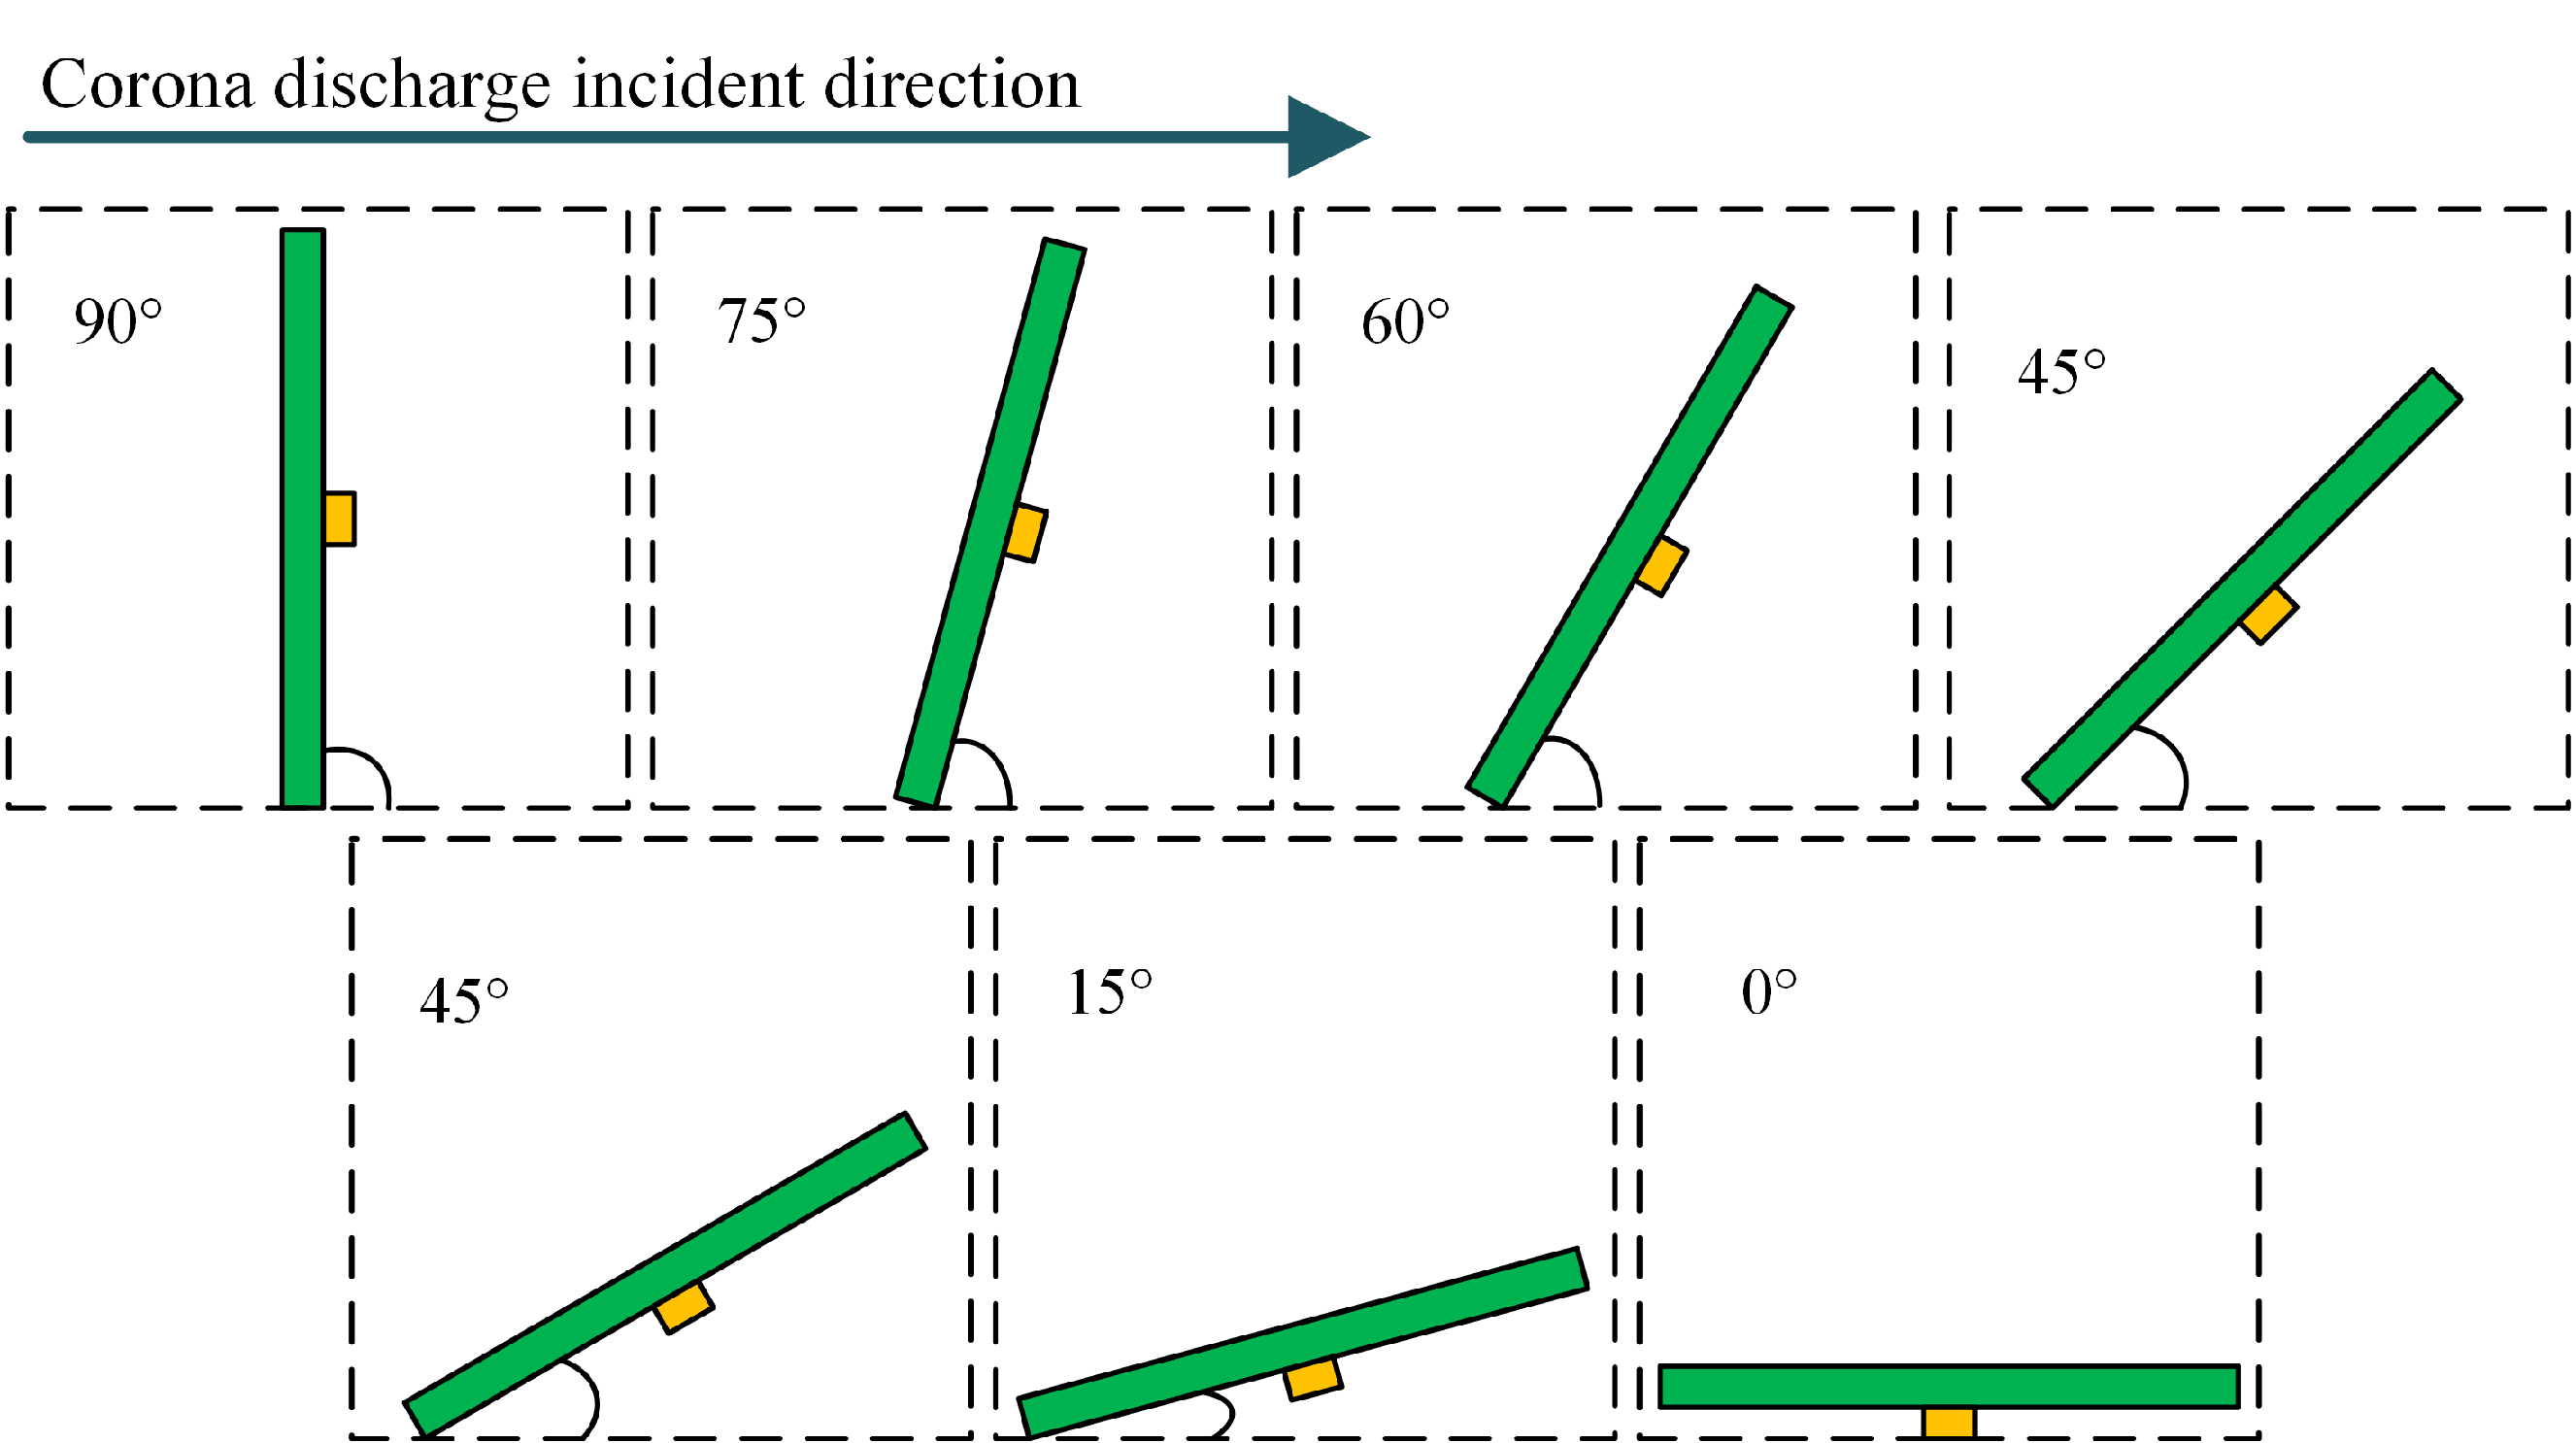
\includegraphics[width=0.8\textwidth]{images/564630268a062c85fb92b70f0c2f667c_p7_i1.png}
    \caption{Plataforma experimental.}
    \end{figure}
    \item \textbf{Pruebas de detección:} Se detectaron señales de descarga de corona a distancias de 1, 4, 7, 10 y 13 m, y también se varió el ángulo de colocación de la antena (0° a 90° en incrementos de 15°) para evaluar el efecto de la dirección de la onda incidente (Figura \ref{fig:placement_angle}).
    \begin{figure}[htpb]
    \centering
    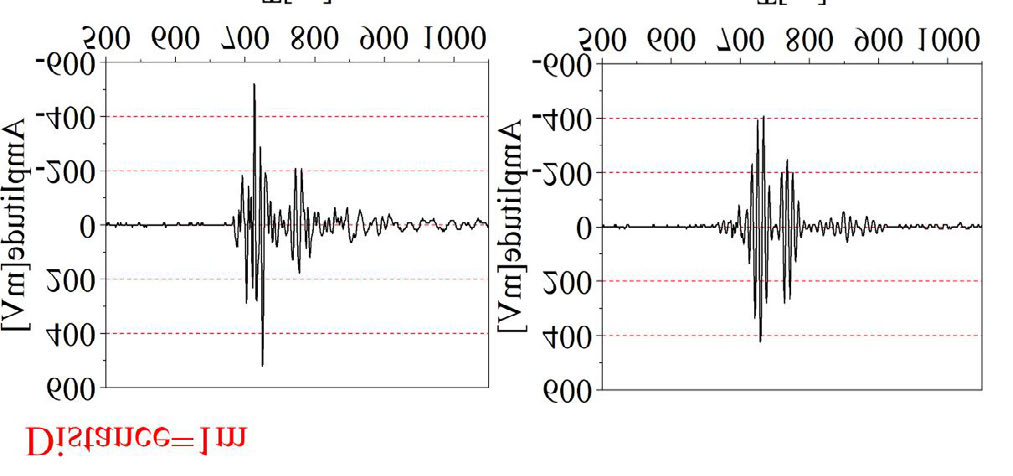
\includegraphics[width=0.8\textwidth]{images/564630268a062c85fb92b70f0c2f667c_p7_i10.jpeg}
    \caption{Esquemático del cambio del ángulo de colocación de la antena.}
    \end{figure}
    \item \textbf{Medición de carga:} Se utilizó una bobina de Rogowski de alta frecuencia para medir la capacidad de carga liberada por el circuito experimental.
\end{itemize}

\subsection*{Resultados o hallazgos}

\textbf{1. Rendimiento de la FSS:}
\begin{itemize}
    \item La FSS diseñada mostró una curva S11 < -10 dB en el rango de frecuencia de 100–500 MHz (Figura \ref{fig:fss_s11_final}), con una frecuencia resonante de 248 MHz. Esto indica una absorción de más del 90\% de la onda electromagnética en la banda de interés.
    \begin{figure}[htpb]
    \centering
    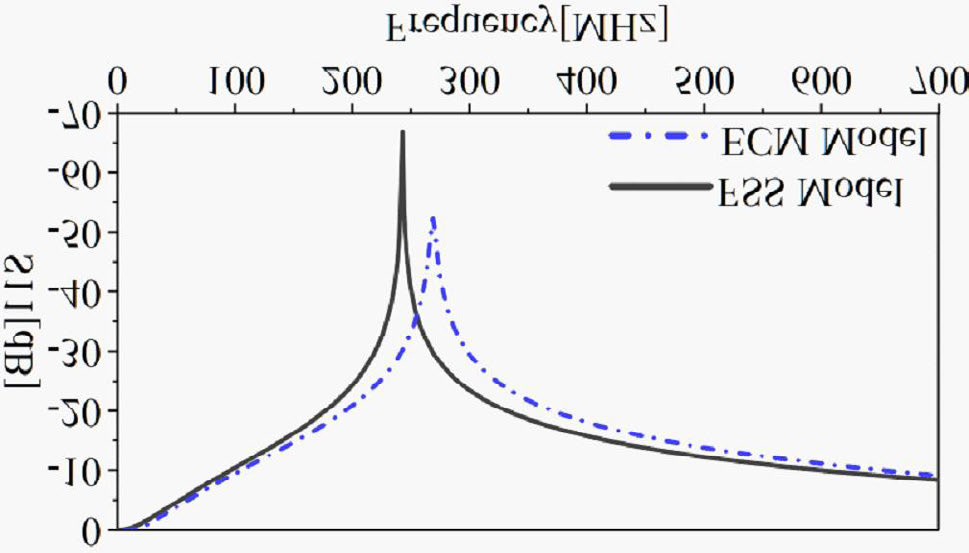
\includegraphics[width=0.8\textwidth]{images/564630268a062c85fb92b70f0c2f667c_p4_i4.jpeg}
    \caption{(c) Curva S11 de la FSS de doble capa con inductores de chip y su circuito equivalente.}
    \end{figure}
    \item El análisis de Monte Carlo (Figura \ref{fig:monte_carlo_s11}) reveló que la tolerancia del inductor afecta significativamente el parámetro S11 de la FSS a 248 MHz, pero el impacto es menor a 100 y 500 MHz, lo que confirma su influencia en la frecuencia resonante.
    \begin{figure}[htpb]
    \centering
    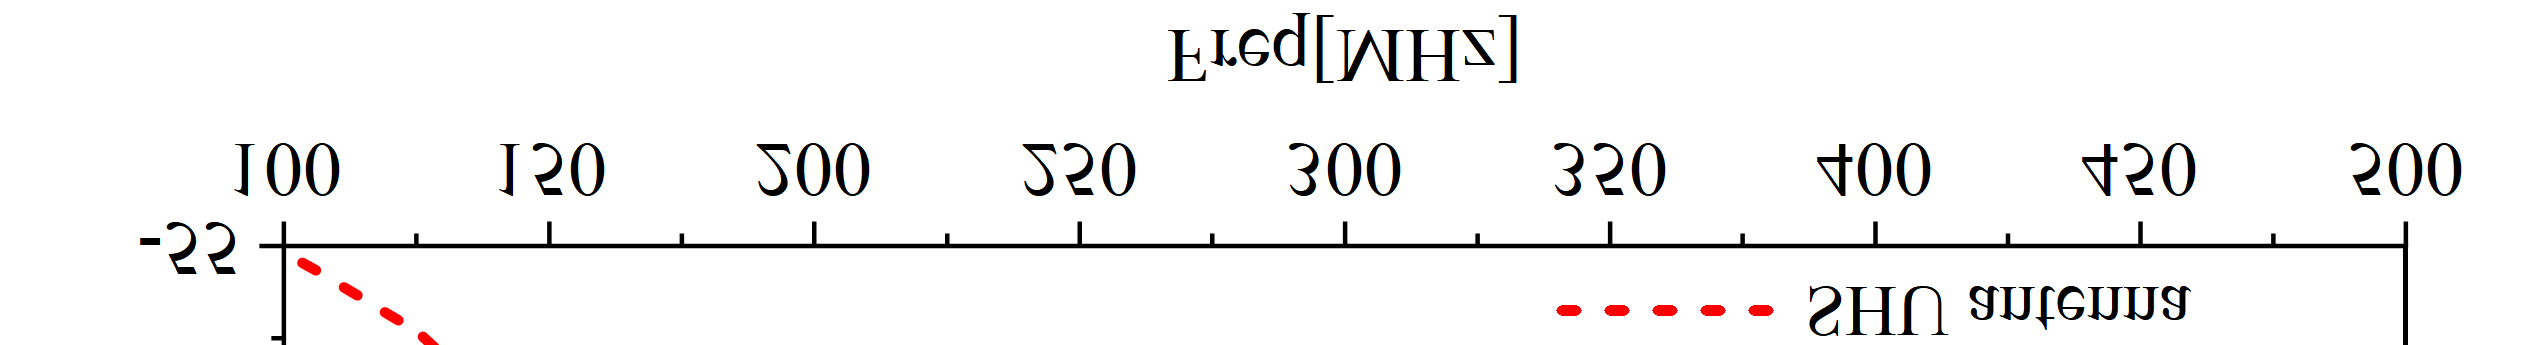
\includegraphics[width=0.8\textwidth]{images/564630268a062c85fb92b70f0c2f667c_p5_i1.png}
    \caption{(a) Curva S11 de la FSS. (b) Histograma de la distribución S11 a 100 MHz. (c) Histograma de la distribución S11 a 248 MHz. (d) Histograma de la distribución S11 a 500 MHz.}
    \end{figure}
\end{itemize}

\textbf{2. Rendimiento de la antena FSHU (FSS-SHU):}
\begin{itemize}
    \item \textbf{Distancia óptima (h):} La simulación mostró que la FSS puede mejorar la capacidad de la antena para recibir ondas electromagnéticas, siendo óptima una distancia 'h' de 20 mm entre la FSS y la antena SHU. A esta altura, la curva S11 de la antena FSHU es significativamente más baja que la de la antena SHU (Figura \ref{fig:fshu_s11_heights}), y la ganancia de la antena se maximiza (Figura \ref{fig:gain_comparison}).
    \begin{figure}[htpb]
    \centering
    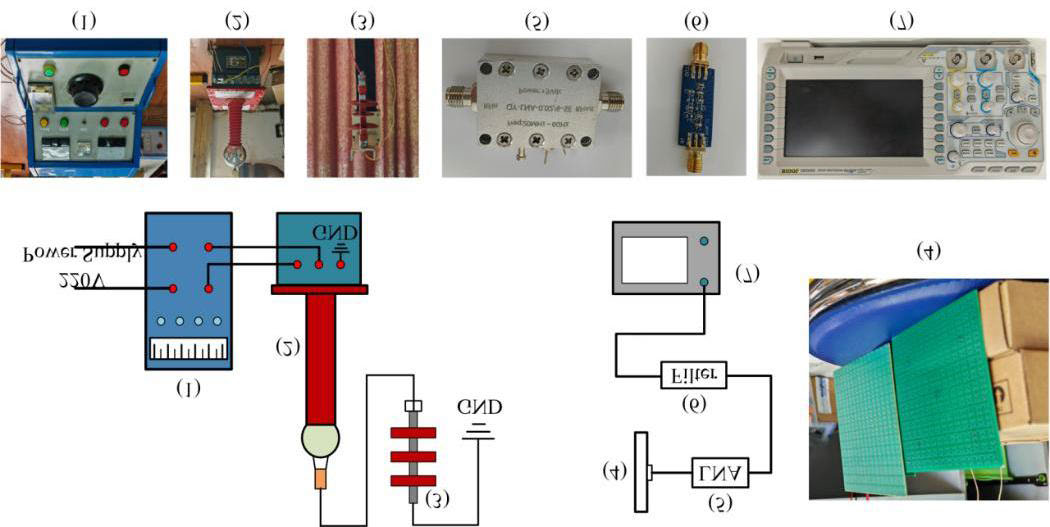
\includegraphics[width=0.8\textwidth]{images/564630268a062c85fb92b70f0c2f667c_p6_i1.jpeg}
    \caption{Curva S11 de la antena global para diferentes alturas.}
    \end{figure}
    \begin{figure}[htpb]
    \centering
    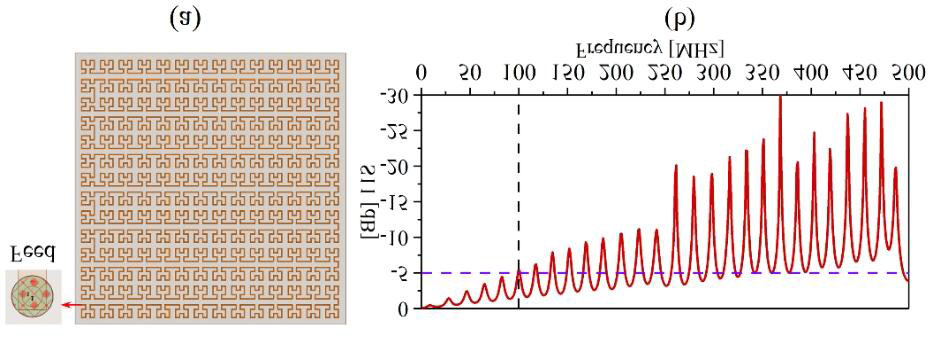
\includegraphics[width=0.8\textwidth]{images/564630268a062c85fb92b70f0c2f667c_p5_i5.jpeg}
    \caption{Comparación de ganancia de antenas.}
    \end{figure}
    \item \textbf{Amplitud de la señal:} La antena FSHU detectó amplitudes de señal de descarga de corona 128\%, 130\%, 132\% y 135\% más altas que la antena SHU a distancias de 1, 4, 7 y 10 m, respectivamente.
    \item \textbf{Distancia máxima de detección:} La antena FSHU alcanzó una distancia máxima de detección de 13 m, donde la antena SHU ya no podía detectar la señal (Figura \ref{fig:corona_signals_distances}).
    \begin{figure}[htpb]
    \centering
    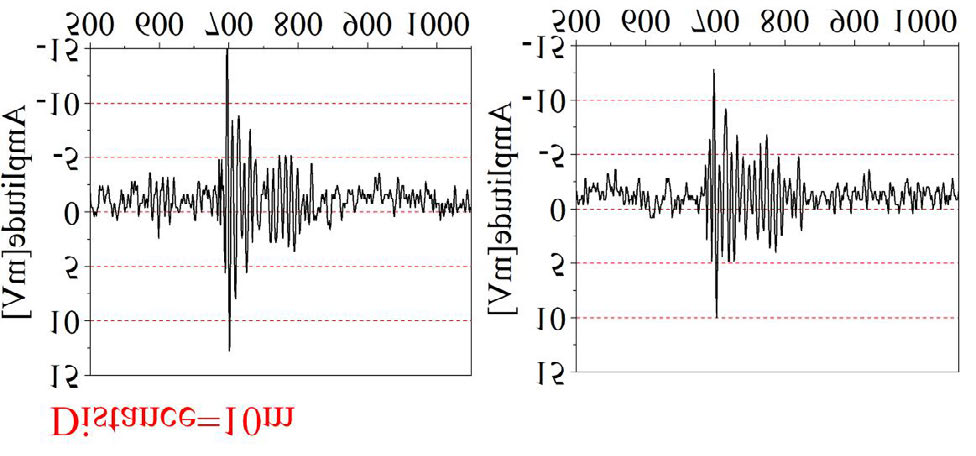
\includegraphics[width=0.8\textwidth]{images/564630268a062c85fb92b70f0c2f667c_p7_i4.jpeg}
    \caption{(a) Ruido ambiental. (b) Distancia de detección de 1 m. (c) Distancia de detección de 4 m. (d) Distancia de detección de 7 m. (e) Distancia de detección de 10 m. (f) Distancia de detección de 13 m.}
    \end{figure}
    \item \textbf{Efecto del ángulo:} La amplitud de la señal disminuyó a medida que el ángulo de incidencia se reducía. A 10 m, la FSHU no pudo detectar señales a 0°, y a 13 m, solo pudo detectar a 90° (Figura \ref{fig:amplitude_vs_angle}).
    \begin{figure}[htpb]
    \centering
    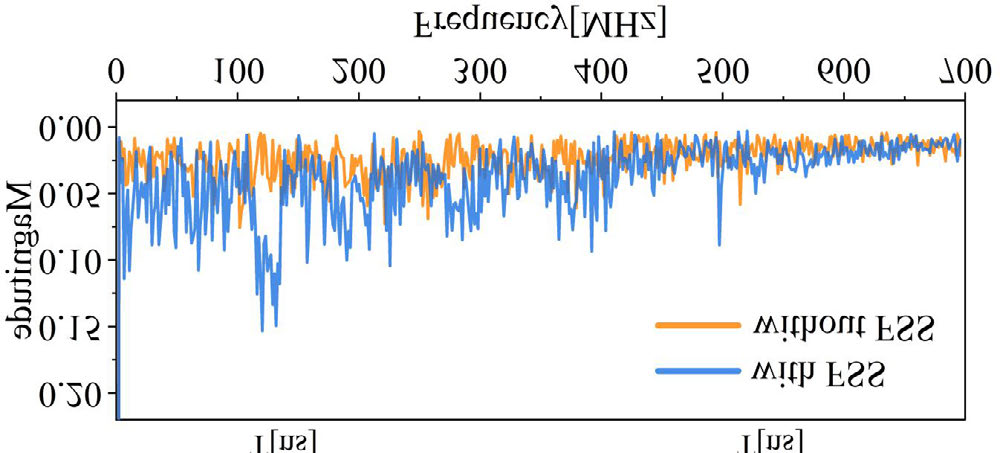
\includegraphics[width=0.8\textwidth]{images/564630268a062c85fb92b70f0c2f667c_p7_i11.jpeg}
    \caption{Amplitud promedio de la antena a diferentes distancias correspondiente al cambio en el ángulo de la antena. (a) 1 m, (b) 4 m, (c) 7 m y (d) 10 m.}
    \end{figure}
\end{itemize}

\textbf{3. Comparación con trabajos previos:}
La antena FSHU diseñada presenta una distancia de detección óptima de 13 m, superando a otras antenas en la literatura que son significativamente más grandes y menos portátiles, como se detalla en la Tabla \ref{tab:comparison_table}.

\begin{table}[htpb]
\centering
\caption{Comparación con otros trabajos}
\begin{tabular}{|c|c|c|}
\hline
\textbf{Ref. No.} & \textbf{Tamaño} & \textbf{Distancia de detección} \\
\hline
{[}7{]} & 2x4 m (superficie de recepción) & 320m \\
{[}8{]} & Diámetro: 360 mm, Altura: 2284 mm & 260m \\
{[}10{]} & 100mm$\times$100mm$\times$1.6mm & 5m \\
\textbf{Este trabajo} & \begin{tabular}{c} 130mm$\times$130mm$\times$1.6mm con \\ 150mm$\times$150mm$\times$1.6mm \end{tabular} & \textbf{13m} \\
\hline
\end{tabular}
\end{table}

\subsection*{Discusión o análisis crítico}

El principio de funcionamiento de la FSS para mejorar la sensibilidad se basa en un efecto de multicapa. La FSS, al ser una estructura electromagnética artificial compuesta de celdas periódicamente arregladas, refleja y transmite selectivamente las ondas electromagnéticas. Al superponerla sobre la antena de detección, la onda electromagnética incidente atraviesa la FSS, se convierte en una onda saliente, una parte es capturada por la antena y el resto se refleja. Esta onda reflejada incide nuevamente en la parte trasera de la FSS, que la vuelve a reflejar hacia la antena, repitiendo este ciclo. Este proceso cíclico aumenta la cantidad total de ondas electromagnéticas capturadas por la antena, mejorando su sensibilidad.

Aunque los resultados de simulación y experimentales muestran una clara mejora en la sensibilidad y el alcance de detección de la antena FSHU en comparación con la SHU original, existen algunas discrepancias entre las curvas S11 simuladas y las medidas. Esto se atribuye principalmente a:
\begin{itemize}
    \item La soldadura manual de la interfaz SMA en el punto de alimentación, que introduce inductancia y reactancia adicionales en la antena.
    \item La presencia de ruido electromagnético de alta frecuencia en el entorno de detección, como la interferencia electromagnética vehicular, que afecta la precisión de la detección.
\end{itemize}
Estos factores, aunque impactan la precisión, no invalidan la mejora general lograda por la FSS.

La miniaturización es un aspecto clave de este diseño, permitiendo que la antena sea portátil y adecuada para su uso con UAVs. A pesar de su tamaño compacto, la antena FSHU logra una distancia de detección de 13 m, que es superior a otras antenas pequeñas existentes. Sin embargo, el diseño actual aún presenta desafíos:
\begin{itemize}
    \item \textbf{Ganancia de la antena:} Se requiere una mejora adicional en la ganancia de la antena. Esto podría lograrse optimizando la forma de la capa de microstrip.
    \item \textbf{Peso:} El material del sustrato dieléctrico utilizado (FR4) contribuye al peso de la antena. Para futuras aplicaciones, especialmente en UAVs, se podrían considerar materiales de baja densidad como el tereftalato de polietileno (PET) para reducir el peso.
\end{itemize}

\subsection*{Conclusiones o implicaciones}

En este artículo, se diseñó con éxito una FSS de banda ancha (100–500 MHz) para mejorar la sensibilidad de una antena de detección de descarga de corona. La FSS consta de dos parches: una capa superior de celdas cruzadas retorcidas y una capa inferior de celdas cruzadas con elementos inductivos. Las simulaciones confirmaron que la FSS exhibe un S11 < -10 dB en la banda de frecuencia objetivo y que una distancia de 20 mm entre la FSS y la antena de detección optimiza el rendimiento.

Los experimentos de descarga de corona validaron que la antena FSHU (SHU con FSS) mejora significativamente la capacidad de capturar ondas electromagnéticas, con amplitudes de señal entre 128\% y 135\% más altas que la antena SHU sin FSS en rangos de 1 a 10 m. Además, la antena FSHU logró la detección más lejana de 13 m, superando a la antena SHU que no pudo detectar a esa distancia. Este trabajo demuestra el potencial de las FSS para mejorar la detección de descargas de corona, ofreciendo una solución más sensible y de mayor alcance para la inspección de líneas de transmisión de alto voltaje.

\subsection*{Síntesis final}
Este estudio presenta una antena miniaturizada (FSHU) mejorada con una Superficie Selectiva en Frecuencia (FSS) para la detección de descarga de corona. La FSS de doble capa, diseñada para 100-500 MHz, se superpuso a una antena fractal de Hilbert serpentina (SHU). Los resultados experimentales muestran un aumento de hasta 135\% en la amplitud de la señal y una distancia máxima de detección de 13 m, superando a la antena SHU original y a otros diseños previos, lo que mejora la precisión y seguridad en el monitoreo de líneas de alto voltaje.

\newpage
% --- Inicio del documento: sensors-19-04255.pdf ---
\section{Design and Application of a Metamaterial Superstrate on a Bio-Inspired Antenna for Partial Discharge Detection through Dielectric Windows}

\subsection*{Contexto y objetivo}
El monitoreo continuo de las descargas parciales (DP) en equipos de alta tensión es crucial para prevenir la degradación del aislamiento y fallas del equipo. El método tradicional IEC 60270 es invasivo. El método radiométrico o de Ultra Alta Frecuencia (UHF) es una alternativa no invasiva, detectando ondas electromagnéticas emitidas por las DP en el rango de 300 MHz a 3 GHz. Las antenas monopolo impresas (PMA) son adecuadas para esto debido a su bajo costo, patrones de radiación atractivos, amplio ancho de banda y facilidad de construcción, pero las PMA tradicionales suelen ser grandes y requieren una alta ganancia para detectar DP de baja intensidad.

Este trabajo se basa en una PMA bioinspirada (basada en la hoja de \textit{Jatropha mollissima}) desarrollada previamente, que ya cumple con los requisitos de tamaño, ancho de banda y ganancia para la detección de DP a través de ventanas dieléctricas. El objetivo principal de este estudio es diseñar un superestrato de metamaterial, utilizando ventanas dieléctricas existentes, para mejorar la sensibilidad de detección de DP de esta PMA bioinspirada. Se busca mejorar específicamente la ganancia, el ancho de banda y el patrón de radiación de la antena mediante la incorporación de resonadores de anillo dividido (SRR) y tiras de carga capacitivas (CLS) en el superestrato dieléctrico.

\subsection*{Metodología o desarrollo}
La metodología se dividió en tres etapas: procedimientos computacionales, pruebas experimentales de laboratorio y aplicación en campo.

\subsubsection*{Procedimientos Computacionales}
Se utilizó el software HFSS (High Frequency Structure Simulator) para el diseño y simulación. El sustrato empleado fue FR-4 con $\varepsilon_r = 4.4$, un espesor $h = 1.6$ mm y una tangente de pérdidas $\delta = 0.02$. Las simulaciones se realizaron en un rango de frecuencia de 200 MHz a 1600 MHz.

\begin{itemize}
    \item \textbf{Diseño de la PMA Bioinspirada}: Se utilizó una estructura basada en la hoja de \textit{Jatropha mollissima} (Pohl) Baill, cuyas dimensiones finales se muestran en la Figura \ref{fig:PMA_design}.
    \begin{figure}[htpb]
    \centering
    
\includegraphics[width=0.8\textwidth]{images/f1c5b012cd86bd42b78fd9b9b77f9e22_p7_i2.png}
    \caption{PMA bioinspirada: detalles del modelo final diseñado (todas las dimensiones en centímetros) \cite{26}.}
    \end{figure}
    \item \textbf{Simulaciones de Celdas Unitarias de Metamaterial}: Se diseñaron y evaluaron estructuras SRR-CLS rectangulares y circulares para exhibir propiedades de doble negatividad (DNG) en el rango de frecuencia de actividad de DP (300--1500 MHz). Las dimensiones de estas celdas unitarias se presentan en la Figura \ref{fig:SRR_cells}.
    \begin{figure}[htpb]
    \centering
    
\includegraphics[width=0.8\textwidth]{images/f1c5b012cd86bd42b78fd9b9b77f9e22_p8_i1.jpeg}
    \caption{Modelos SRR para cada celda unitaria de metamaterial (las tiras verdes son las estructuras CLS): (a) rectangular.}
    \end{figure}
    Para la caracterización como metamateriales, cada modelo se simuló individualmente bajo condiciones de contorno específicas (paredes de conductor eléctrico perfecto (PEC) y de conductor magnético perfecto (PMC)), excitado por dos puertos de onda (Waveports), como se ilustra en la Figura \ref{fig:boundary_conditions}. Esto permitió la obtención de los coeficientes $S_{11}$ y $S_{21}$ para calcular la permitividad ($\varepsilon$) y permeabilidad ($\mu$) efectivas.
    \begin{figure}[htpb]
    \centering
    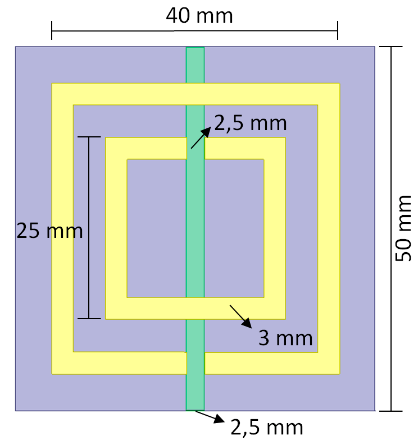
\includegraphics[width=0.8\textwidth]{images/f1c5b012cd86bd42b78fd9b9b77f9e22_p8_i3.png}
    \caption{Condiciones de contorno para los modelos SRR-CLS simulados.}
    \end{figure}
    \item \textbf{Simulaciones de Superestrato de Metamaterial}: Las celdas unitarias caracterizadas se posicionaron en una matriz de 3x3 como superestratos sobre la PMA bioinspirada, como se muestra en la Figura \ref{fig:superstrates}.
    \begin{figure}[htpb]
    \centering
    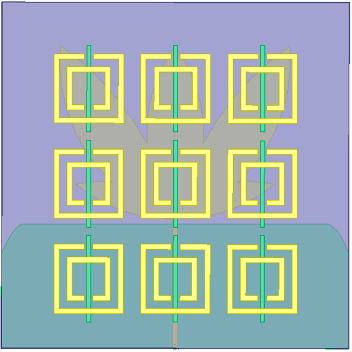
\includegraphics[width=0.8\textwidth]{images/f1c5b012cd86bd42b78fd9b9b77f9e22_p9_i1.png}
    \caption{Superestratos de metamaterial posicionados sobre la PMA bioinspirada: (a) rectangular.}
    \end{figure}
    La altura óptima del superestrato se definió en 135 mm para los SRR rectangulares y 125 mm para los circulares. Los espaciamientos entre celdas se ajustaron a 10x15 mm (rectangular) y 8x14 mm (circular), con una separación de 5 mm en las CLS. También se simuló la PMA solo con el material dieléctrico (FR-4) como superestrato para aislar el efecto del metamaterial.
\end{itemize}

\subsubsection*{Pruebas Experimentales de Laboratorio}
\begin{itemize}
    \item \textbf{Mediciones de Coeficiente de Reflexión y Ganancia}: Los valores del coeficiente de reflexión ($S_{11}$) se obtuvieron con un analizador de redes ENA E5062A. Las mediciones de ganancia se realizaron en una cámara anecoica con una antena de referencia (Hyperlog 30100X, 4.5 dBi de ganancia media) y la antena bajo prueba (AUT), como se esquematiza en la Figura \ref{fig:gain_setup}. La distancia al campo lejano (R) se estableció en 1.0 m. La ganancia de la antena bajo prueba ($G_D$) se calculó utilizando una ecuación de Friis adaptada.
    \begin{figure}[htpb]
    \centering
    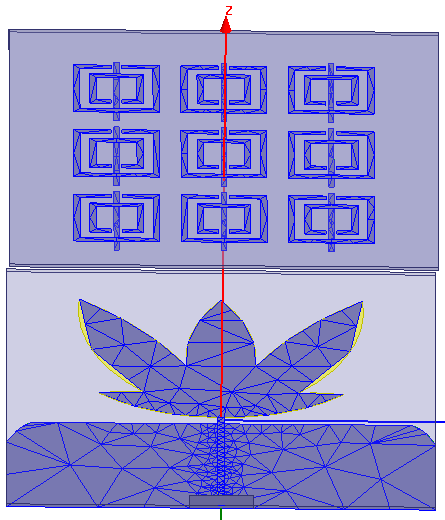
\includegraphics[width=0.8\textwidth]{images/f1c5b012cd86bd42b78fd9b9b77f9e22_p10_i1.png}
    \caption{Esquema de la configuración experimental utilizada en la prueba de medición de ganancia.}
    \end{figure}
    \item \textbf{Pruebas de Sensibilidad de Detección de DP}: Se utilizó una celda de aceite (configuración de electrodo punto-a-plano con disco de poliamida) como generador de DP, conectada a un capacitor de acoplamiento (1000 pF) y un circuito resonante (LDM-5). El montaje experimental se muestra en la Figura \ref{fig:PD_setup}. Las pulsos de DP se adquirieron con un osciloscopio Keysight DSO90604A. Se realizaron procedimientos de calibración según la norma IEC 60270 para correlacionar la carga aparente de DP con los valores de voltaje medidos.
    \begin{figure}[htpb]
    \centering
    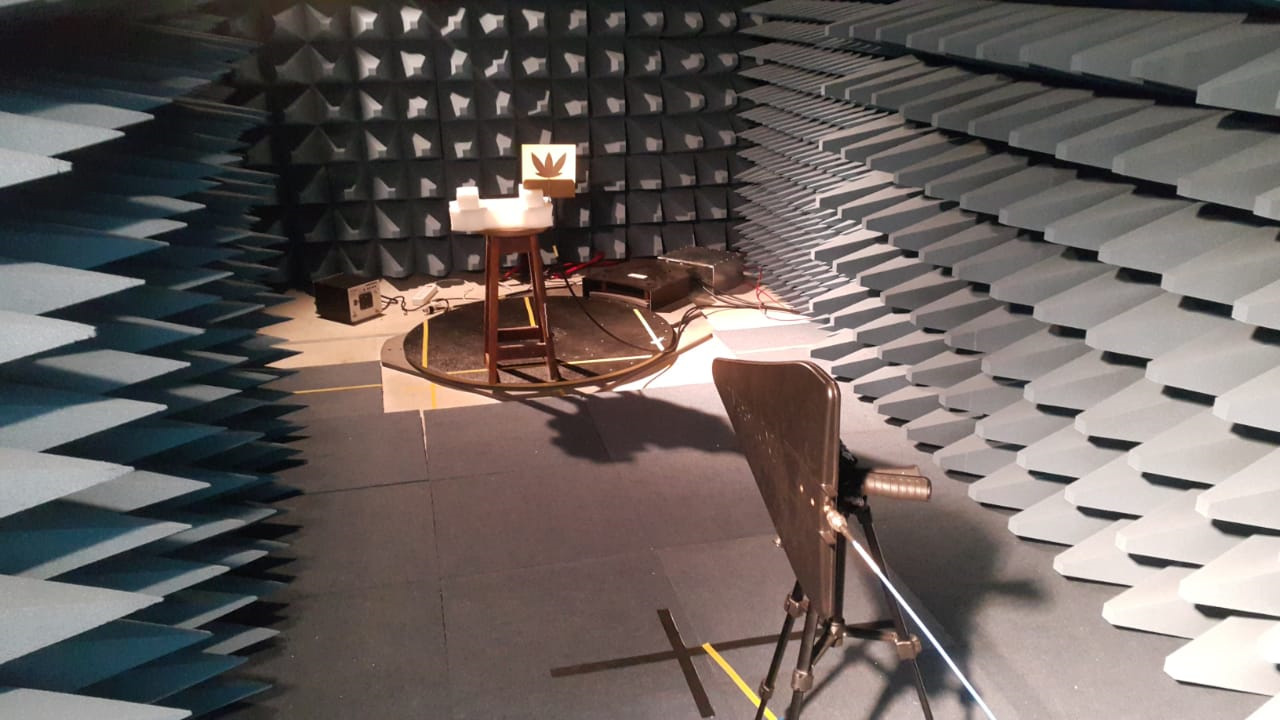
\includegraphics[width=0.8\textwidth]{images/f1c5b012cd86bd42b78fd9b9b77f9e22_p11_i1.jpeg}
    \caption{Configuración experimental aplicada para la medición de Descarga Parcial (PD).}
    \end{figure}
\end{itemize}

\subsubsection*{Aplicación en Campo}
El conjunto PMA-metamaterial se probó en un Transformador de Corriente (TC) de 230 kV en una subestación brasileña (Mussuré II). Este TC fue seleccionado por su degradación del aislamiento. Los pulsos de DP se adquirieron en el dominio del tiempo con un osciloscopio Tektronix TDS5104B. Para fines comparativos, la PMA bioinspirada sin superestrato también se utilizó simultáneamente a la misma distancia del TC. Un generador de señales se usó para producir una tensión de referencia sinusoidal y así identificar las señales de DP por su ubicación de fase y periodicidad. El TC se muestra en la Figura \ref{fig:CT_field}.
\begin{figure}[htpb]
\centering
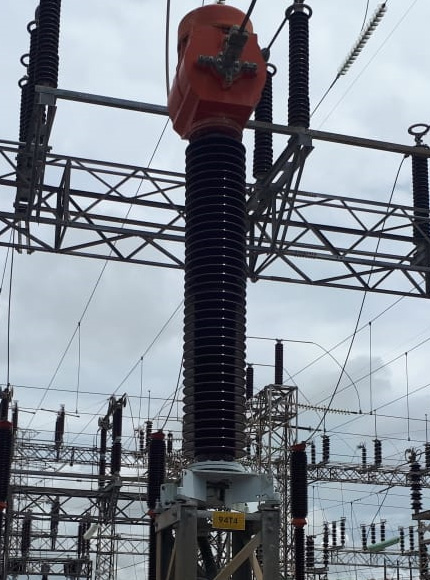
\includegraphics[width=0.8\textwidth]{images/f1c5b012cd86bd42b78fd9b9b77f9e22_p12_i1.jpeg}
\caption{El Transformador de Corriente de 230 kV evaluado en las pruebas de aplicación en campo.}
\end{figure}

\subsection*{Resultados o hallazgos}

\subsubsection*{Resultados de la Simulación}
\begin{itemize}
    \item \textbf{Ganancia de la PMA Bioinspirada}: La ganancia máxima simulada de la PMA bioinspirada mostró valores por debajo del umbral recomendado (2 dBi) para frecuencias cercanas a la frecuencia de operación inferior (487 MHz), como se observa en la Figura \ref{fig:PMA_gain_sim}.
    % [Imagen omitida porque no se encontró el archivo: f1c5b012cd86bd42b78fd9b9b77f9e22_p13_i1.png]
    \item \textbf{Coeficientes de Reflexión de Celdas Unitarias de Metamaterial}: Las celdas unitarias circulares y rectangulares presentaron anchos de banda dentro del rango de actividad de DP, operando hasta 1033 MHz y 1117 MHz, respectivamente.
    \item \textbf{Valores de $\mu$ y $\varepsilon$ de Celdas Unitarias}: Ambas celdas unitarias de metamaterial exhibieron características de doble negatividad ($\varepsilon < 0$ y $\mu < 0$) en casi todo el rango de actividad de DP (300--1500 MHz), con la excepción de bandas específicas (1190--1350 MHz para SRR rectangular y 1100--1300 MHz para SRR circular) donde $\mu$ fue positiva. La Figura \ref{fig:meta_mu_eps} muestra un ejemplo para la celda circular.
    % [Imagen omitida porque no se encontró el archivo: f1c5b012cd86bd42b78fd9b9b77f9e22_p14_i7.png]
    \item \textbf{Influencia del Superestrato en el Coeficiente de Reflexión}: La aplicación del superestrato (con o sin metamaterial) provocó desplazamientos en la frecuencia de operación inferior de la PMA. El superestrato de FR4 (sin metamaterial) mostró un desplazamiento de 42 MHz (reducción de ancho de banda del 5.2\%). Con el metamaterial, los desplazamientos fueron de 56 MHz (rectangular) y 77 MHz (circular). También hubo un aumento de la frecuencia superior (22 MHz para rectangular, 64 MHz para circular), resultando en una reducción total del ancho de banda del 3.9\% y 1.8\% respectivamente. Se observaron mejoras en los coeficientes de reflexión para el rango de 1050--1300 MHz (por debajo de -10 dB). La Figura \ref{fig:S11_comparison_sim} ilustra esta comparación.
    \begin{figure}[htpb]
    \centering
    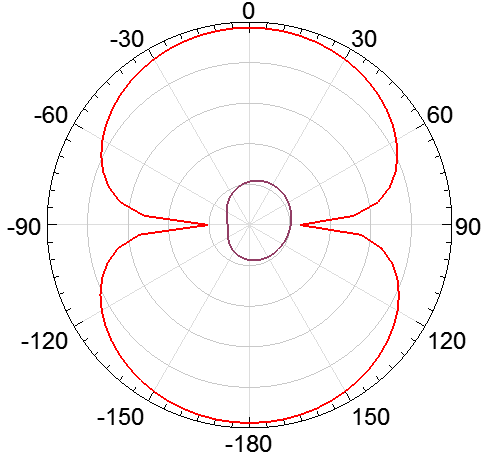
\includegraphics[width=0.8\textwidth]{images/f1c5b012cd86bd42b78fd9b9b77f9e22_p15_i1.png}
    \caption{Comparación entre los coeficientes de reflexión de las estructuras simuladas.}
    \end{figure}
    \item \textbf{Patrones de Radiación}: La adición del superestrato de FR4 no alteró significativamente los patrones de radiación de la PMA. Sin embargo, los superestratos SRR introdujeron distorsiones en los patrones de radiación en las frecuencias de operación superiores (Figuras 22-24 del documento original), siendo el SRR rectangular el que presentó menores distorsiones. Los patrones fueron adecuados para aplicaciones en ventanas dieléctricas, con la mayoría de los valores de radiación máxima concentrados en la dirección de acoplamiento (0°).
    \item \textbf{Ganancia Máxima}: La aplicación de ambos superestratos (SRR rectangular y circular) resultó en valores de ganancia máxima casi duplicados respecto a la PMA de referencia en el rango de 500--1000 MHz. El SRR circular también mostró una mejora significativa en el rango de 1300--1500 MHz. La ganancia fue superior a 2 dBi en todo el rango de 500--1500 MHz con la adición del metamaterial. La Figura \ref{fig:max_gain_comparison_sim} muestra la comparación. La ganancia media simulada para la PMA de referencia fue de 2.81 dBi, para el FR4 superestrato de 2.83 dBi, para el SRR rectangular de 3.96 dBi y para el SRR circular de 4.07 dBi. El SRR rectangular se seleccionó para las pruebas experimentales debido a su mejor relación ganancia/ancho de banda/patrón de radiación.
    % [Imagen omitida porque no se encontró el archivo: f1c5b012cd86bd42b78fd9b9b77f9e22_p17_i4.png]
\end{itemize}

\subsubsection*{Resultados Experimentales de Laboratorio}
\begin{itemize}
    \item \textbf{Antenas Fabricadas}: Se construyeron la PMA bioinspirada sin superestrato y con superestrato de metamaterial SRR rectangular, como se muestra en la Figura \ref{fig:PMA_manufactured}.
    \begin{figure}[htpb]
    \centering
    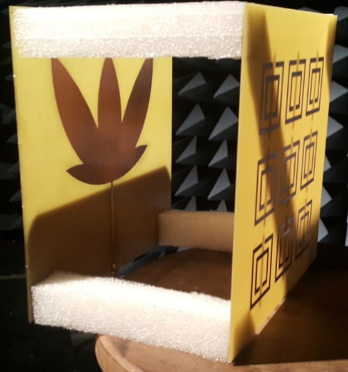
\includegraphics[width=0.8\textwidth]{images/f1c5b012cd86bd42b78fd9b9b77f9e22_p18_i2.jpeg}
    \caption{PMA bioinspirada fabricada: (b) con superestrato de metamaterial.}
    \end{figure}
    \item \textbf{Coeficientes de Reflexión Medidos}: Los resultados medidos y simulados mostraron un comportamiento similar. Para la PMA sin metamaterial, el ancho de banda medido fue de 472 MHz hasta valores superiores a 1500 MHz. Con el metamaterial, la frecuencia inferior se desplazó a 540 MHz (un desplazamiento de 68 MHz), y se verificó un mejor rendimiento del coeficiente de reflexión en el rango de 1.1–1.5 GHz. La Figura \ref{fig:S11_measured_sim} muestra la comparación.
    % [Imagen omitida porque no se encontró el archivo: f1c5b012cd86bd42b78fd9b9b77f9e22_p18_i3.png]
    \item \textbf{Ganancia Medida}: Las curvas de ganancia medidas y simuladas coincidieron en su comportamiento. La PMA sin metamaterial presentó una ganancia media medida de 2.92 dBi. Con el superestrato de metamaterial, la ganancia media medida fue de 3.61 dBi, lo que representa una mejora de 0.7 dBi. Esto resultó en una antena con valores de ganancia superiores a 2 dBi desde 575 MHz hasta 1.5 GHz, indicando una alta sensibilidad para la detección de DP. La Figura \ref{fig:gain_measured_sim} presenta la comparación.
    % [Imagen omitida porque no se encontró el archivo: f1c5b012cd86bd42b78fd9b9b77f9e22_p19_i1.png]
    \item \textbf{Sensibilidad de Detección de DP}: El conjunto PMA-metamaterial detectó exitosamente todos los pulsos de DP generados en la celda de aceite (Figura \ref{fig:PD_pulses_lab}), que también fueron detectados por el método IEC 60270. Los voltajes medidos en los terminales de la antena fueron aproximadamente la mitad de los obtenidos por el método estándar. Las DP detectadas mostraron cargas aparentes entre 15 y 60 pC, un rango típico para DP de baja intensidad. Un espectrograma de los pulsos de DP (Figura \ref{fig:PD_spectrogram}) confirmó concentraciones de energía espectral hasta 1500 MHz, validando la cobertura del rango de frecuencia de interés (300--1500 MHz).
    % [Imagen omitida porque no se encontró el archivo: f1c5b012cd86bd42b78fd9b9b77f9e22_p20_i1.png]
    \begin{figure}[htpb]
    \centering
    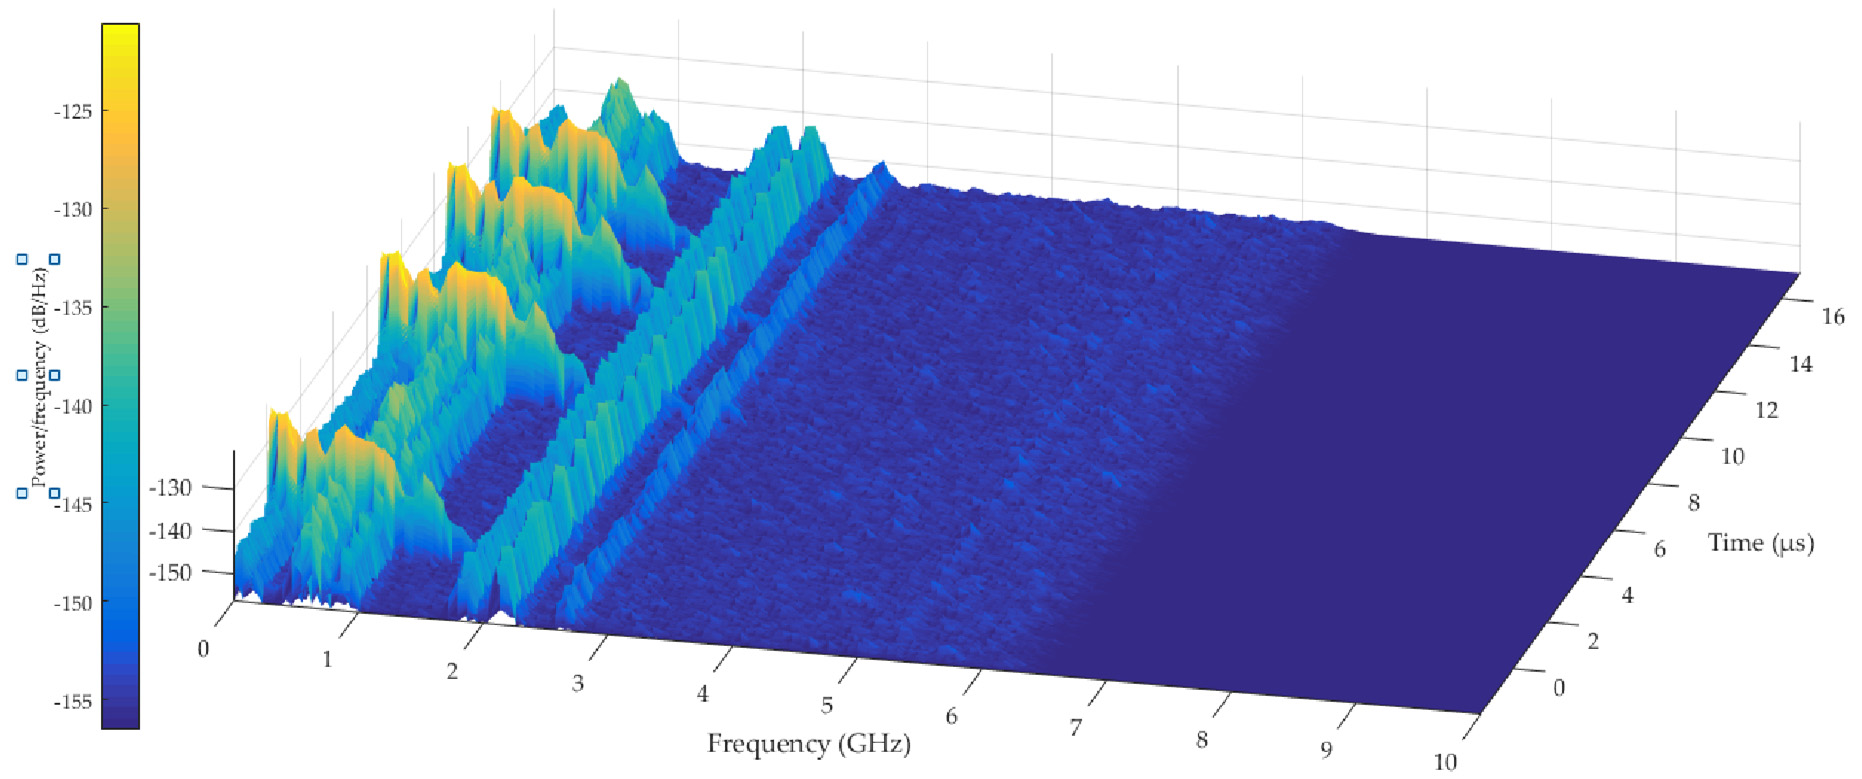
\includegraphics[width=0.8\textwidth]{images/f1c5b012cd86bd42b78fd9b9b77f9e22_p21_i1.jpeg}
    \caption{Espectrograma de la muestra de pulsos de DP detectada por el conjunto PMA-metamaterial bioinspirado presentado en la Figura \ref{fig:PD_pulses_lab}.}
    \end{figure}
\end{itemize}

\subsubsection*{Detección de DP en Subestación de 230 kV}
\begin{itemize}
    \item \textbf{Detección de DP}: El conjunto PMA-metamaterial detectó exitosamente señales con características de DP (transiciones de medio ciclo de tensión sinusoidal de referencia y desplazamiento de fase de aproximadamente 180° entre pulsos), como se muestra en la Figura \ref{fig:PD_pulses_field}. Presentó una mayor sensibilidad de detección, con amplitudes de señal casi duplicadas en comparación con la PMA de referencia sin superestrato.
    % [Imagen omitida porque no se encontró el archivo: f1c5b012cd86bd42b78fd9b9b77f9e22_p21_i2.png]
    \item \textbf{Sensibilidad Práctica}: Se confirmó un nivel considerable de DP en el TC, lo que atestigua la sensibilidad práctica de la antena desarrollada para la detección de DP. No fue posible estimar los niveles de carga aparente de DP en campo debido a limitaciones prácticas.
\end{itemize}

\subsection*{Discusión o análisis crítico}
La integración del superestrato de metamaterial con la PMA bioinspirada ha demostrado ser una solución viable para mejorar la detección de DP. En comparación con antenas más competitivas como las Hornet o Vivaldi (Tabla 3 del documento original) que ofrecen mayor ganancia, el conjunto PMA-metamaterial presenta una ventaja significativa en sus dimensiones (200 mm $\times$ 200 mm $\times$ 135 mm) y facilidad de instalación en ventanas dieléctricas de equipos de alta tensión. Mientras que otras antenas de alta ganancia son considerablemente más grandes, el diseño propuesto logra una ganancia media de 3.61 dBi y un ancho de banda de 500--1500 MHz, características que son adecuadas para la detección de DP.

Aunque el método no permitió estimar la carga aparente de DP en las pruebas de campo, la capacidad de evaluar la evolución de la actividad de DP mediante la tensión inducida en los terminales de la antena es una valiosa información para el monitoreo continuo, no invasivo y de bajo costo. El trabajo futuro se centrará en técnicas de calibración, clasificación y localización para caracterizar completamente el sensor para diagnóstico de equipos de DP.

\subsection*{Conclusiones o implicaciones}
Las conclusiones principales de este estudio son:
\begin{enumerate}
    \item Ambas celdas unitarias SRR-CLS diseñadas mostraron un comportamiento de doble negatividad ($\mu < 0$, $\varepsilon < 0$) en casi todo el rango de frecuencia principal de actividad de DP (300--1500 MHz), clasificándolas como metamateriales aplicables como superestrato.
    \item La aplicación del superestrato de metamaterial resultó en desplazamientos en el rango de frecuencia de operación de la PMA, con reducciones de ancho de banda del 3.9\% para SRR rectangular y 1.8\% para SRR circular.
    \item A pesar de la reducción del ancho de banda, la aplicación de los superestratos de metamateriales resultó en valores de coeficiente de reflexión más altos para el rango de 1100--1500 MHz, mejorando la capacidad de transmisión/recepción de potencia de la antena.
    \item Se observaron distorsiones en los patrones de radiación en las frecuencias de operación superiores de la PMA para ambos superestratos de metamaterial, siendo el SRR rectangular el que presentó menores distorsiones, especialmente en la dirección del lóbulo posterior.
    \item La aplicación de ambos superestratos diseñados resultó en un aumento de la ganancia máxima casi al doble en el rango de frecuencia de 500--1000 MHz, con una mejora de la ganancia media superior a 1 dBi.
    \item La aplicación práctica del superestrato SRR rectangular resultó en un sensor UHF con un ancho de banda operativo (540--1500 MHz) que cubre el 80\% del rango de frecuencia principal de actividad de DP (300--1500 MHz).
    \item La ganancia media medida para el conjunto PMA-metamaterial fue de 3.61 dBi, lo que representa una mejora de 0.7 dBi respecto a la PMA bioinspirada de referencia (2.92 dBi) y una buena sensibilidad de detección de DP.
    \item En las pruebas de laboratorio de DP, el conjunto PMA-metamaterial bioinspirado fue capaz de detectar cargas aparentes superiores a 15 pC.
    \item La PMA bioinspirada presentó valores de voltaje medidos con la mitad de la magnitud obtenida del método estándar IEC 60270, resultando en una alta sensibilidad de detección de DP para un método radiométrico.
    \item Finalmente, el conjunto PMA-metamaterial bioinspirado demostró ser eficaz en la aplicación práctica de detección de DP en un TC de 230 kV.
\end{enumerate}

\subsection*{Síntesis final}
Este estudio diseñó y aplicó exitosamente un superestrato de metamaterial en una antena monopolo impresa (PMA) bioinspirada para mejorar la detección de descargas parciales (DP) en sistemas de alta tensión a través de ventanas dieléctricas. La integración de resonadores de anillo dividido (SRR) y tiras de carga capacitivas (CLS) resultó en un aumento significativo de la ganancia media de la antena a 3.61 dBi (una mejora de 0.7 dBi) y mantuvo un ancho de banda de operación adecuado (540-1500 MHz). Las pruebas de laboratorio y de campo confirmaron la alta sensibilidad y eficacia del conjunto PMA-metamaterial para detectar DP, posicionándolo como un sensor UHF optimizado, no invasivo y de bajo costo para el monitoreo continuo.

\end{document}
